\documentclass[11pt,a4paper]{report}

\hbadness=10000
\hfuzz=100pt

\usepackage{tablefootnote}
\usepackage[utf8]{inputenc}
\usepackage[hidelinks]{hyperref} 
\usepackage[T1]{fontenc}
\usepackage[top=2cm,bottom=2cm,left=2.5cm,right=2.5cm]{geometry}
\usepackage{amsmath,amsfonts,amssymb}
\usepackage{graphicx}
\usepackage{subcaption}
\usepackage{caption}
\usepackage{inconsolata}
\usepackage{array}
\usepackage{color}
\usepackage{tcolorbox}
\usepackage{fancyhdr}
\usepackage[export]{adjustbox}
\usepackage[english]{babel}
\usepackage{listings}
\usepackage{hyperref}
\usepackage{transparent}
\usepackage{eso-pic}
\usepackage{chngpage}
\usepackage{shorttoc}
\usepackage{comment}
\usepackage{makeidx}
\usepackage[backend=biber]{biblatex}
\addbibresource{bibliographie/biblio.bib}
\usepackage{csquotes}
\usepackage{multirow}
\usepackage{footnotehyper}
\usepackage{xcolor}
\usepackage{acro}
\usepackage{pgfplots}
\usepackage{ragged2e}
\usepackage{tabularx}
\usepackage{float}
\usepackage{microtype}
\usepackage{chngcntr}
\usepackage{tocloft}
\usepackage{nicefrac}
\usepackage{titlesec}  % pour styliser section*

\usepackage{dirtree}
\usepackage[absolute,overlay]{textpos}

\usepackage{enumitem}

\usepackage{algorithm}
\usepackage{algpseudocode}
\usepackage{mathtools}    % amélioration de amsmath
\usepackage{bm}           % pour les vecteurs/matrices en gras

%\usepackage[linesnumbered,ruled,vlined]{algorithm2e}
\usepackage{dsfont}           % Pour les ensembles (ex : indicatrice)

%\usepackage[T1]{fontenc}\usepackage{textcomp}
%\usepackage{mathpazo}
%\usepackage{courier}
%\usepackage{url,ngerman}

%\usepackage[inactive]{pst-pdf}

%\usepackage{pstricks,pst-node}
%\newcounter{leaves}
%\newcounter{directories}

\usepackage{forest}

\definecolor{folderbg}{RGB}{124,166,198}
\definecolor{folderborder}{RGB}{110,144,169}

\def\Size{4pt}
\tikzset{
  folder/.pic={
    \filldraw[draw=folderborder,top color=folderbg!50,bottom color=folderbg]
      (-1.05*\Size,0.2\Size+5pt) rectangle ++(.75*\Size,-0.2\Size-5pt);  
    \filldraw[draw=folderborder,top color=folderbg!50,bottom color=folderbg]
      (-1.15*\Size,-\Size) rectangle (1.15*\Size,\Size);
  },
  file/.pic={
    \draw[fill=white, draw=black] (0,0) rectangle (1*\Size,1*\Size);
    \node at (0.5*\Size, 0.5*\Size) {
\includegraphics[width=0.4cm]{images/other/file.png}};
  }
}


%\forestset{
%  declare toks={directory icon}{\includegraphics[height=1em]{images/folder.png}},
%  declare toks={file icon}{
\includegraphics[height=1em]{images/file.png}},
%  file/.style={label=right:{\file icon}},
%  directory/.style={label=right:{\directory icon}},
%}

\begin{comment}
%\usepackage{forest}
\usepackage[edges]{forest}
% Définition du style 'pic dir tree'
\forestset{
  pic dir tree/.style={
    for tree={
      grow'=0,
      child anchor=west,
      parent anchor=south,
      anchor=west,
      calign=first,
      inner sep=1pt,
      l sep=10pt,
      edge path={
        \noexpand\path [draw, \forestoption{edge}] (!u.parent anchor) -- (.child anchor)\forestoption{edge label};
      },
      if n children=0{
        tier=word,
        label={},
      }{},
      before typesetting nodes={
        if n=1{folder}{file},
      },
    },
  },
  file/.style={font=\ttfamily, inner sep=2pt},
  folder/.style={font=\ttfamily\bfseries, inner sep=2pt},
}


\forestset{folder icons}
\end{comment}

\usepackage{tikz-qtree}

\usepackage{siunitx}


\usepackage[super]{nth}

\usepackage[table]{xcolor}


%\counterwithin{table}{section}
%\renewcommand{\thetable}{\thesection.\arabic{table}} % Format table number as section.table
%\renewcommand{\thefigure}{\thesection.\arabic{figure}} % Format figure number as section.figure
% Command to refer to an appendix item as "Annexe n"
\newcommand{\annexref}[1]{annexe~\ref{#1}}

\newcounter{annex}
\renewcommand{\theannex}{\arabic{annex}}

\newcommand{\annex}[2]{%
  \refstepcounter{annex}%
  \section*{Annex \theannex\ -- #1}%
  \label{#2}%
  \addcontentsline{toc}{section}{Annex \theannex\ -- #1}
}

\usetikzlibrary{patterns}
\pgfplotsset{compat=1.17}

\setlength{\parskip}{0.5\baselineskip}


\DeclareAcronym{U-RANS}{
  short = U-RANS,
  long = Unsteady Reynolds-Averaged Navier–Stokes,
  short-indefinite = une,
}

\DeclareAcronym{OpenFOAM}{
  short = OpenFOAM,
  long = Open source Field Operation And Manipulation,
  short-indefinite = un,
}

\DeclareAcronym{MPI}{
  short = MPI,
  long = Message Passing Interface,
  short-indefinite = un,
}

\DeclareAcronym{MRF}{
  short = MRF,
  long = Multiple Reference Frame,
  short-indefinite = un,
}

\DeclareAcronym{SST}{
  short = SST,
  long = Shear Stress Transport,
  short-indefinite = le,
}

\DeclareAcronym{SHF}{
  short = SHF,
  long = "Société Hydrotechnique de France",
  short-indefinite = la,
}

\DeclareAcronym{JFM}{
  short = JFM,
  long = Journal of Fluid Mechanics,
  short-indefinite = le,
}

\DeclareAcronym{CPER}{
  short = CPER,
  long = "Contrat de Plan État-Région",
  short-indefinite = un,
}

\DeclareAcronym{HCERES}{
  short = HCERES,
  long = "Haut Conseil de l'Évaluation de la Recherche et de l'Enseignement Supérieur",
  short-indefinite = le,
}

\DeclareAcronym{CTI}{
  short = CTI,
  long = "Commission des Titres d'Ingénieur",
  short-indefinite = une,
}

\DeclareAcronym{DDRS}{
  short = DDRS,
  long = "Développement Durable et Responsabilité Sociétale",
  short-indefinite = le,
}

\DeclareAcronym{CTES}{
  short = CTES,
  long = "Convention pour la Transition des Établissements du Supérieur",
  short-indefinite = une,
}

\DeclareAcronym{NRMSE}{
  short = NRMSE,
  long = Normalized Root Mean Square Error,
  short-indefinite = une,
}

\DeclareAcronym{DNS}{
  short = DNS,
  long = Direct Numerical Simulation,
  short-indefinite = une,
}

\DeclareAcronym{CFL}{
  short = CFL,
  long = Courant-Friedrichs-Lewy,
  short-indefinite = un,
}

\DeclareAcronym{AI}{
  short = AI,
  long = Artificial Intelligence,
  short-indefinite = une,
}

\DeclareAcronym{DA}{
  short = DA,
  long = Data Assimilation,
  short-indefinite = une,
}

\DeclareAcronym{RSU}{
  short = RSU,
  long = "Rapport Social Unique",
  short-indefinite = un,
}

\DeclareAcronym{CHSCTN}{
  short = CHSCTN,
  long = {"Comité d'Hygiène, de Sécurité et des Conditions de Travail National"},
  short-indefinite = un,
}

\DeclareAcronym{EnKF}{
  short = EnKF,
  long = Ensemble Kalman Filter,
  short-indefinite = un,
}

\DeclareAcronym{LES}{
  short = LES,
  long = Large Eddy Simulation,
  short-indefinite = une,
}

\DeclareAcronym{RANS}{
  short = RANS,
  long = Reynolds-Averaged Navier–Stokes equations,
  short-indefinite = une,
}

\DeclareAcronym{PIV}{
  short = PIV,
  long = Particle Image Velocimetry,
  short-indefinite = une,
}

\DeclareAcronym{IBM}{
  short = IBM,
  long = Immersed Boundary Methods,
  short-indefinite = une,
}

\DeclareAcronym{IPSA}{
  short = IPSA,
  long = "Institut Polytechnique des Sciences Avancées",
  short-indefinite = un,
}

\DeclareAcronym{CONES}{
  short = CONES,
  long = Coupling OpenFoam with Numerical EnvironmentS,
  short-indefinite = un,
}

\DeclareAcronym{ENSAM}{
  short = ENSAM,
  long = "École Nationale Nupérieure d'Arts et Métiers",
  short-indefinite = une,
}

\DeclareAcronym{LMFL}{
  short = LMFL,
  long = "Laboratoire de Mécanique des Fluides de Lille",
  short-indefinite = un,
}

\DeclareAcronym{ONERA}{
  short = ONERA,
  long = "Office National d'Études et de Recherche Aérospatiales",
  short-indefinite = un,
}

\DeclareAcronym{CFD}{
  short = CFD,
  long = Computation Fluid Dynamics, %, pour mécanique des fuides numérique {}
  short-indefinite = un,
}

\DeclareAcronym{TGCC}{
  short = TGCC,
  long = "Très Grand Centre de Calcul du CEA",
  short-indefinite = un,
}

\DeclareAcronym{CEA}{
  short = CEA,
  long = "Commissariat à l'Énergie Atomique",
}

% ACRONYMS STAGE CERFACS M1

\DeclareAcronym{CNES}{
  short = CNES,
  long = "Centre National d'Études Spatiales",
  short-indefinite = un,
}

\DeclareAcronym{CNRS}{
  short = CNRS,
  long = "Centre National de la Recherche Scientifique",
  short-indefinite = un,
}

\DeclareAcronym{EDF}{
  short = EDF,
  long = "Électricité De France",
  short-indefinite = une,
}

%\DeclareAcronym{ONERA}{
%  short = ONERA,
%  long = Office National d'Études et de Recherche Aérospatiales ,
%  short-indefinite = un,
%}

\DeclareAcronym{SAS}{
  short = SAS,
  long = "Société par Actions Simplifiées",
  short-indefinite = une,
}

\DeclareAcronym{SI}{
  short = SI,
  long = "Système International d'unités",
  short-indefinite = un,
}

\DeclareAcronym{KDTree}{
  short = KDTree,
  long = {"K-Dimensional Tree, pour arbre à k-dimensions"},
  short-indefinite = un,
}

\DeclareAcronym{Mo}{
  short = Mo,
  long = "Mégaoctets",
  short-indefinite = un,
}

\DeclareAcronym{RBF}{
  short = RBF,
  long = {Radial Basis Function, pour fonction de base radiale},
  short-indefinite = une,
}

\DeclareAcronym{MLS}{
  short = MLS,
  long = {Moving Least Squares, pour moindres carrés mobiles},
  short-indefinite = une,
}

\DeclareAcronym{MISCOG}{
  short = MISCOG,
  long = {Multi-Instance Solver Coulpled trough Overlapping Grids, pour Solveur multi-instances couplées à travers des grilles superposées}, % ou couplé ?????
  short-indefinite = une,
}


\DeclareAcronym{DSM}{
  short = DSM,
  long = {Digital Surface Model, pour modèle numérique de surface},
  short-indefinite = une,
}

\DeclareAcronym{1D}{
  short = 1D,
  long = "une Dimension",
  short-indefinite = Une,
}

\DeclareAcronym{GIP}{
  short = GIP,
  long = "Groupement d’Intérêt Public",
  short-indefinite = un,
}

%\DeclareAcronym{CFD}{
%  short = CFD,
%  long = {Computation Fluid Dynamics, pour mécanique des fuides numérique},
%  short-indefinite = un,
%}

\DeclareAcronym{CSR}{
  short = CSR,
  long = Corporate Social Responsibility,
  short-indefinite = une,
}

\DeclareAcronym{RSE}{
  short = RSE,
  long = "Responsabilité Sociétale des Entreprises",
  short-indefinite = une,
}

\DeclareAcronym{CERFACS}{
  short = CERFACS,
  long = "Centre Européen de Recherche et de Formation Avancée en Calcul Scientifique",
  short-indefinite = un,
}

\DeclareAcronym{HPC}{
  short = HPC,
  long = {High Performance Computing, pour calcul haute performance},
  short-indefinite = un,
}

\DeclareAcronym{IDW}{
  short = IDW,
  long = {"Inverse Distance Weighting, pour pondération inverse à la distance"},
  short-indefinite = une,
}

\DeclareAcronym{FWH}{
  short = FWH,
  long = Ffowcs Williams-Hawkings,
  short-indefinite = une,
}

\DeclareAcronym{NURBS}{
  short = NURBS,
  long = {Non Uniform Rational Basis Splines, pour B-splines rationnelles non uniformes},
  short-indefinite = une,
}


\DeclareAcronym{CAO}{
  short = CAO,
  long = "Conception Assistée par Ordinateur",
  short-indefinite = une,
}

\DeclareAcronym{QVT}{
  short = QVT,
  long = "Qualité de Vie au Travail",
  short-indefinite = la,
}

\DeclareAcronym{CSE}{
  short = CSE,
  long = "Comité Social et Économique",
  short-indefinite = le,
}

\DeclareAcronym{CSSCT}{
  short = CSSCT,
  long = {"Commission Santé, Sécurité et Conditions de Travail"},
  short-indefinite = la,
}

\DeclareAcronym{DUERP}{
  short = DUERP,
  long = "Document Unique d’Évaluation des Risques Professionnels",
  short-indefinite = le,
}

\DeclareAcronym{OTP}{
  short = OTP,
  long = One-Time-Password,
  short-indefinite = le,
}

\DeclareAcronym{DSP}{
  short = DSP,
  long = "Densité spectrale de puissance",
  short-indefinite = le,
}

\DeclareAcronym{ALGO-COOP}{
  short = ALGO-COOP,
  long = {"parallels ALGOrithmes \& sCientifics sOftware Operational Performances, pour algorithmes parallèles et logiciels scientifiques performances opérationnelles"},
  short-indefinite = l',
}

\DeclareAcronym{CSG}{
  short = CSG,
  long = {Computer Service General, pour équipe informatique et support utilisateur},
  short-indefinite = le,
}

\DeclareAcronym{ES}{
  short = ES,
  long = {Energy and Safety, pour énergie et sécurité},
  short-indefinite = l',
}

\DeclareAcronym{AAM}{
  short = AAM,
  long = {Advanced Aerodynamics and Multiphysics, pour aérodynamique avancée et multiphysique},
  short-indefinite = l',
}

\DeclareAcronym{GLOBC}{
  short = GLOBC,
  long = {modelling climate and GLOBal Change, pour modélisation du climat et de son changement global},
  short-indefinite = la,
}

\DeclareAcronym{RGPD}{
  short = RGPD,
  long = "Règlement Général sur la Protection des Données",
  short-indefinite = le,
}


\lstset{ 
    language=Python,                     % Langage
    basicstyle=\ttfamily\footnotesize,   % Style de base
    keywordstyle=\color{blue},           % Style des mots-clés
    commentstyle=\color{green},          % Style des commentaires
    stringstyle=\color{red},             % Style des chaînes de caractères
    numbers=left,                        % Numérotation des lignes
    numberstyle=\tiny\color{gray},       % Style des numéros de ligne
    stepnumber=1,                        % Numérotation chaque ligne
    numbersep=5pt,                       % Distance entre les numéros de ligne et le code
    showspaces=false,                    % Ne pas afficher les espaces
    showstringspaces=false,              % Ne pas afficher les espaces dans les chaînes de caractères
    tabsize=4,                           % Taille des tabulations
    captionpos=b,                        % Position des légendes (en bas)
    breaklines=true,                     % Retour à la ligne automatique
    breakatwhitespace=false,             % Retour à la ligne uniquement dans les espaces
    frame=single,                        % Cadre autour du code
    framerule=0.5pt,
    rulecolor=\color{black},
}
\renewcommand{\lstlistingname}{Code}

\newcommand{\dps}{\displaystyle}

\pagestyle{fancy}
%\renewcommand{\chaptermark}[1]{\markboth{#1}{}}
%\fancyhead[C]{\leftmark} % Affiche le titre du chapitre courant au centre


\setlength{\headheight}{25.22153pt}
\setlength{\footskip}{37.6175pt}

\definecolor{backcolour}{rgb}{0.96,0.96,0.95}
\definecolor{lightbrown}{rgb}{0.71, 0.40, 0.11}
\definecolor{myblue}{rgb}{0.3,0.4,0.9}
\definecolor{green}{rgb}{0.0, 0.5, 0.0}
\definecolor{aurometalsaurus}{rgb}{0.43, 0.5, 0.5}
\definecolor{babyblue}{rgb}{0.54, 0.81, 0.94}
\definecolor{bronze}{rgb}{0.8, 0.5, 0.2}
\definecolor{brilliantrose}{rgb}{1.0, 0.33, 0.64}
\definecolor{darkblue}{RGB}{0, 70, 127}
\definecolor{lightblue}{RGB}{173, 216, 230}
\definecolor{white}{RGB}{255, 255, 255}

\definecolor{myBlue}{rgb}{0.0, 0.45, 0.74}    % similaire à matplotlib blue
\definecolor{myOrange}{rgb}{0.85, 0.33, 0.1}  % similaire à matplotlib orange
\definecolor{myGreen}{rgb}{0.47, 0.67, 0.19}  % similaire à matplotlib green

\newcommand{\bluelinePython}{\textcolor{myBlue}{\rule[0.5ex]{1.5em}{1pt}}}
\newcommand{\orangeline}{\textcolor{myOrange}{\rule[0.5ex]{1.5em}{1pt}}}
\newcommand{\greenline}{\textcolor{myGreen}{\rule[0.5ex]{1.5em}{1pt}}}

\fancypagestyle{plain}{
  \fancyhead[L]{End-of-study thesis \\ Clément THIBAULT}
  \fancyhead[R]{\includegraphics*[width=0.25\textwidth]{images/logo/logos.png}}
  \fancyfoot[C]{page \thepage}
  \fancyfoot[R]{\includegraphics*[width=0.1\textwidth]{images/logo/ipsagarde.png}}
}

\fancyhead[L]{End-of-study thesis \\ Clément THIBAULT}
\fancyhead[R]{\includegraphics*[width=0.25\textwidth]{images/logo/logos.png}}
\fancyfoot[C]{page \thepage}
\renewcommand{\sectionmark}[1]{\markboth{}{}}
\fancyfoot[R]{\includegraphics*[width=0.1\textwidth]{images/logo/ipsagarde.png}}


  \newcommand\BackgroundPic{
  \put(0 cm, 3.5 cm){
  \parbox[b][0.5\paperheight]{\paperwidth}{
  \centering
  {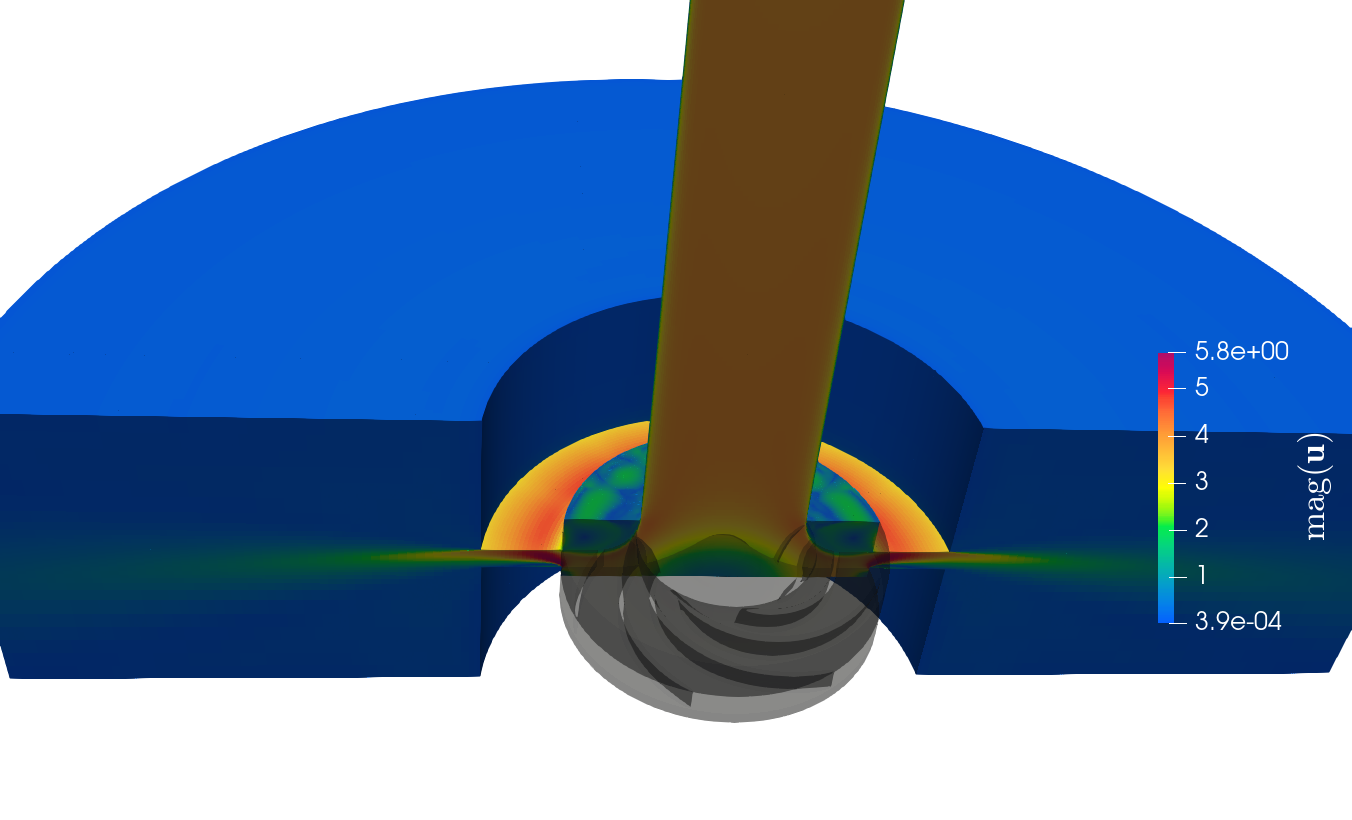
\includegraphics[width=\paperwidth,height=0.32\paperheight, %\transparent{0.4}
  keepaspectratio]{images/numericalPump/Pump_sim2.png}}
  \vspace{2.0cm} % Adjust the spacing between the image and the title
  \makebox[\paperwidth]{\textbf{Cross-section of the pump model}} % Center the title below the image
  }}}

\captionsetup[table]{name=Table}



\begin{document}

\AddToShipoutPicture*{\BackgroundPic}

\begin{titlepage}

    \changepage{3cm}%amount added to textheight
           {}%amount added to textwidth
           {}%amount added to evensidemargin
           {}%amount added to oddsidemargin
           {}%amount added to columnsep
           {-1.5cm}%amount added to topmargin
           {}%amount added to headlight
           {}%amount added to headsep
           {}%amount added to footskip

    
    \parindent=0pt

    \begin{center}
        \renewcommand{\arraystretch}{1.2} % espace entre les lignes
        \begin{tabularx}{\textwidth}{>{\raggedright\arraybackslash}X
                                  >{\centering\arraybackslash}X
                                  >{\raggedleft\arraybackslash}X}
            
\includegraphics[scale=0.28]{images/logo/ipsagarde.png} &
            
\includegraphics[scale=3.1]{images/logo/logo_lmfl-300x138.png} &
            
\includegraphics[scale=0.51]{images/logo/logo-artsEtM-322x84.png} \\
        
            Institut Polytechnique &
            Laboratoire de Mécanique & 
            École Nationale Supérieure \\ [-0.8ex]
        
            Des Sciences Avancées &
            des Fluides de Lille &
            des Arts et Métiers \\
        
            81 Av. de Grande Bretagne &
            8 Bd Louis XIV &
            8 Bd Louis XIV \\ [-0.8ex]
        
            31300 Toulouse &
            59000 Lille &
            59000 Lille \\
        \end{tabularx}
    \end{center}
                

    \vspace*{0.5cm}
    \begin{center}
        \bfseries\LARGE End-of-study thesis for engineering degree
    \end{center}
    \hrulefill
    \begin{center}\bfseries\huge
        Optimization of the performance of a centrifugal pump using Data Assimilation
    \end{center}
    \begin{center}\huge
        Intern in Rotating Machines
    \end{center}

    \vspace*{\stretch{1}}
    \begin{tabbing}
        Clément THIBAULT - Aéro 5 \= \hspace{6cm} \= From February \nth{26}, 2025 \kill
        Educational tutor: Samy LABSIR \\
        Laboratory tutors: Marcello MELDI, Antoine DAZIN, Miguel MARTINEZ VALERO \\
        \\        
        Clément THIBAULT - Aéro 5 \hspace{3cm} From February \nth{26}, 2025 to September \nth{2}, 2025 
        %\phantom{Supervisors: } \\
        %\phantom{Supervisors: }
    \end{tabbing}

    \begin{center}
        Version of \today 
    \end{center}
    
    %\vspace*{1cm}

    
\end{titlepage}

\newpage
\pagenumbering{arabic}
\pagestyle{fancy}
\setcounter{page}{2}

\fancypagestyle{custompage}{
  \fancyhf{} % Clear header/footer
  \fancyhead[L]{Livrable Stage M1 \\ Clément THIBAULT}
  \fancyhead[R]{\includegraphics*[width=0.2\textwidth]{images/logo/ipsagarde.png}}
  \fancyfoot[C]{page 2}
  \fancyfoot[R]{\includegraphics*[width=0.1\textwidth]{images/logo/ipsagarde.png}}
}

\thispagestyle{custompage}

\chapter*{Acknoledgments}

%Je tiens à sincèrement remercier mon maître de stage, Carlos MONTILLA, de m'avoir guidé tout au long de ce stage et toujours aidé avec le sourire.

\vspace{0.5cm}


%Je tiens également à remercier madame la Présidente du CERFACS, Catherine LAMBERT, pour sa sympathie et pour m'avoir permis d'effectuer ce stage. % pour sa bienveillance et pour m'avoir offert l'opportunité de réaliser ce stage.

%Merci à mes amis montagnards et passionnés de mathématiques, Benjamin CANOVAS-ANDRIEUX et Dimitri \mbox{LANIER} ainsi qu'à mon professeur à l'IPSA, Guillaume COUFFIGNAL, pour leur précieuse aide en mathématiques.

%Merci à mon tuteur pédagogique, Nadir MESSAI, pour son aide dans ma recherche de stage et au sein du CERFACS pendant mes douze semaines de stage.

%Merci à Alexis BOUDIN pour ses explications sur l'interpolation d'ordre élevé.
%Merci à mes amis et collègues Kélian RENOUX, Luc POTIER, Arthur COLOMBIÉ, Guillaume DAVILLER ainsi qu'à l'administration et au CSG pour l'aide qu'ils m'ont apportée au cours de ce stage.

First of all, I would like to sincerely thank my three internship supervisors.
I would like to express my gratitude to Miguel VALERO MARTINEZ  for his guidance and support throughout this internship. His expertise and encouragement have been invaluable.
Thank to Marcello for all his expert advices and to integrating me in the lab.
Thank to Antoine for his physical explanations.

[...] "cobureau" Tom for all his very clear explanations

Thank to Paolo for his CONES explanations and precious support.
Thank to Sarp for his hapiness

Thank to ENSAM and LMFL administration
Thank to ... qui m'a payé le stage
Thank to TGCC thak allow me to acced to supercomputers

for their guidance and support throughout this internship. Their expertise and encouragement have been invaluable.

Thank to Samy LABSIR " d'avoir accepté d'être mon tuteur IPSA pour ce stage"


METTRE LE "page 2" à la bonne hauteur


\vspace*{\fill} % Remplir l'espace vertical jusqu'en bas de la page
\begin{center}
    
\includegraphics[width=0.067\textwidth]{images/other/page_2.png}
\end{center}
\vspace*{-13.5cm} % Ajustez cette valeur pour que l'image soit plus proche du bas de la page
\vspace*{\fill} % Remplir l'espace vertical après l'image



\newpage
\tableofcontents % table of contents


\newpage
\section*{Summary sheet}

\addcontentsline{toc}{chapter}{Summary sheet}
%\begin{comment}
The aim of this technical assessment is to summarize the gaps and their causes between the course's missions and what has been achieved.
It also enables us to suggest what could be done by the next person working on the same subject.


\begin{table}[ht]
\centering
\begin{tabular}{|p{6.5cm}|p{8.7cm}|}
\hline

\rowcolor{darkblue}
\multicolumn{2}{|c|}{\color{white}\textbf{Summary sheet}   \hspace{6.5cm}   Clément THIBAULT - Aéro 5 TIE} \\ 

\rowcolor{lightblue}
\hline
\textbf{Internship topic} & \textbf{Objectives} \\ 
\hline



\begin{minipage}[t]{6.5cm}
    Optimization of the performance of a centrifugal pump using Data \\ Assimilation \hspace{0.2cm}
\end{minipage} & 
\begin{minipage}[t]{8.5cm}
%\begin{itemize}
    Optimization of forcing parameters of the IBM using DA with CONES
%\end{itemize}
\end{minipage} \\ 

\rowcolor{lightblue}
\hline
\textbf{Main customer} & \textbf{Used tools} \\ 
\hline
\begin{minipage}[t]{6.5cm}
%\begin{itemize}
- LMFL

- ENSAM \hspace{0.2cm}
%\end{itemize}
\end{minipage} & 
\begin{minipage}[t]{8.5cm}
CONES, VSCode, Python, TGCC, Paraview, Git, OpenFoam (C++), Bash
\end{minipage} \\ 



\rowcolor{lightblue}
\hline
\multicolumn{2}{|l|}{\textbf{Conducted studies}} \\ 
\hline
\multicolumn{2}{|p{14cm}|}{
\begin{minipage}[t]{14cm}
- ...%Influence de paramètres de la méthode d'interpolation IDW

- ...%Différences d'erreur entre la méthode IDW et linéaire

- ...%Optimisation de la rapidité du traitement
\hspace{0.5cm}
\end{minipage}
} \\ 

\rowcolor{lightblue}
\hline
\textbf{Results}\cellcolor{lightblue} & \textbf{Explanation of possible differences}\cellcolor{lightblue}\\ 
\hline
\begin{minipage}[t]{6.5cm}
    

- X

- Y

- Z

%\item Paramètres n \simeq 10 et p \simeq 10 optimaux pour la méthode IDW
%\end{itemize}
\end{minipage} & 
\begin{minipage}[t]{8.5cm}

-X

- Y

- Z
\end{minipage} \\ 

\rowcolor{lightblue}
\hline
\textbf{Encountered difficulties} & \textbf{Work to be continued} \\ 
\hline
\begin{minipage}[t]{6.5cm}
%\begin{itemize}
- Getting to grips with the tools

- Y
%\end{itemize}
\end{minipage} & 
\begin{minipage}[t]{8.5cm}
%\begin{itemize}
%- Optimiser la méthode linéaire pour les maillages prismatiques
- X

- Y


% - Implémenter une méthode plus rapide pour les maillages non-structurés

%\end{itemize}
\end{minipage} \\ 
\hline
\end{tabular}
\end{table}  

\textbf{Note:} Acronymes are define later.

%\end{comment}
\newpage

\newpage

\section*{General Introduction}
\addcontentsline{toc}{chapter}{General Introduction}

Since I was young, I've always been fascinated by fluid mechanics.
I remember watching feathers, birds and planes flying and being amazed by the way they could fly.
I was also interested in the way water flows in rivers and sailing boats. In high school, I began working on plane-related projects and explored them more theoretically through \ac{CFD}.

This fascination led me to study physics and mathematics at university, where I discovered applied mathematics including CFD, \ac{AI} and Kalman Filter.
During my studies, I've become passionated about applied mathematics and fluid mechanics. That's why I did my last internship at the \ac{CERFACS}.
It convinced me to do a thesis in CFD after \ac{IPSA}, my current engeneering school.

The subject proposed by the \ac{LMFL} really suited me: CFD using an open-source library, coupled with AI and experimental data. So it was with enthusiasm that I started this internship on February 26, 2025, in this laboratory for a duration of six months.

The main objective of this internship is to improve the numerical simulation of a centrifugal pump using experimental data through \ac{DA}. This allows to improve the understanding of the physical phenomena involved in the pump's operation and then to optimize its performance.

The LMFL is a public laboratory with about 40 researchers and 25 PhD students, spread over three sites located in Lille (\ac{ENSAM} and \ac{ONERA}) and on the Villeneuve d'Ascq campus (Centrale Lille, \ac{CNRS} and University of Lille).

My main tasks during this internship were:

\vspace{-0.15cm}

\begin{itemize}\setlength\itemsep{0.1em}
    \item Explore and understand the limitations of the baseline \ac{IBM};
    \item Establish the set of sensor signals to be employed as high-fidelity inputs in the DA;
    \item Ensure the convergence of the CFD solution using IBM;
    \item Implemente the DA problem in \ac{OpenFOAM} and \ac{CONES};
    \item Optimize the forcing parameters of the IBM using DA with CONES to correct a non-physical behavior.
\end{itemize}

%\vspace{-0.05cm}

To present the details of my internship work, the manuscript is structured as follows:

\autoref{chap1} introduces the LMFL laboratory and the ENSAM Lille campus, with a focus on the scientific environment and the social/environmental 
responsibility of the host institution. 

\autoref{chap2} presents the context of the study: first the state of the art and the problem investigation, then the pre-processing of the experimental data, and finally the numerical ingredients employed, including the CFD governing equations, the OpenFOAM solver, the EnKF method and the CONES library. 

\autoref{chap3} is dedicated to the application to the centrifugal pump case: the modelling of the pump, the preliminary IBM results, the first simple application of the DA, and finally the analysis of the obtained results. 

The report ends with a conclusion, an appendix section gathering additional technical material, the bibliography, and a list of acronyms. 


\begin{comment}
        \item Introduction to DA problems;
        \item Numerical ingredients of the CFD and DA problems;
        \item Preliminary results using IBM;
        \item Application of DA to the IBM;
        \item Results and perspectives.
    \end{enumerate}
\end{comment}

\newpage 

\chapter{The LMFL Laboratory}
%\chapter{CERFACS : Le fondement des logiciels de simulation numérique}
%\chapter*{Le CERFACS : Le fondement des logiciels de simulation numérique}
%\addcontentsline{toc}{chapter}{Le CERFACS : Le fondement des logiciels de
                                %simulation numérique}

% Faire les sous parties


%Le plan doit être dynamique : le lecteur doit ressentir une progression entre le début et la fin du rapport. Ainsi, la « présentation de l’entreprise » (partie I) doit permettre de mieux comprendre la « présentation du travail réalisé » (partie II). En effet, les choix industriels, les processus de fabrication, les méthodes de travail, l’organisation et la culture de l’entreprise, notamment en matière de responsabilité sociétale et de développement durable ( annexe IV, p. 39), ont nécessairement une incidence sur le travail
%du stagiaire.

% \section{Structure du CERFACS}

% \label{actionnaires}

The LMFL is a public laboratory under supervision of Centrale Lille, Université Lille 1, Arts et Métiers Paris Tech, ONERA and CNRS.

\begin{figure}[H]
    \centering
    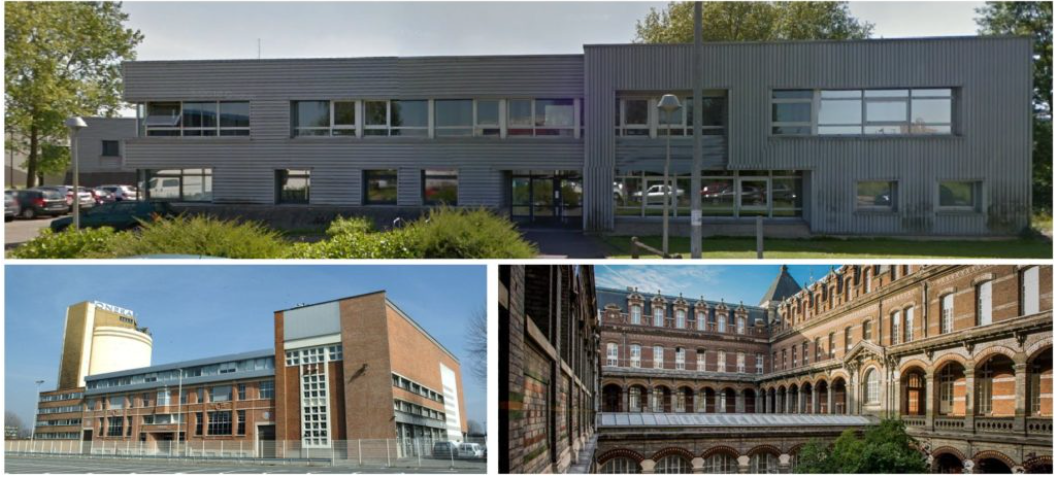
\includegraphics[width=0.90\textwidth]{images/LMFL_facilities.png}
    \caption{LMFL facilities; Top:Villeneuve d’Ascq’s campus gathering Centrale Lille,
    CNRS and Univsersité de Lille. Bottom-left: ONERA. Bottom-right: ENSAM (source : \href{https://lmfl.cnrs.fr/le-laboratoire/}{lmfl.cnrs.fr})}
    %\label{fig:autocorrelation}
\end{figure}



During the last six months, I have been hosted by École Nationale Supérieure des Arts et
Métiers (ENSAM), more precisely at Lille campus. Arts et Métiers is known to be a
prestigious engineering school with a focus on mechanics, industrial and energy engineering.
Its Lille campus offers students unique opportunities to study in a dynamic and innovative
environment, located in the heart of a region known for its industrial history.

This research structure was created on January 1, 2018 by the merger of two research units: the “Écoulements tournants et turbulents” team at the Lille Mechanics Laboratory, and the “Expérimentation et Limite de Vol” research unit.


% (Algorithmes Parallèles \& sCientifics sOftware Operational Performances)
% (Équipe Informatique et Support Utilisateur)
% (Energy et Safety)
% (Advanced Aerodynamics and Multiphysics)
% (Modélisation du climat et de son changement global)

% \section{Mon équipe}

This diversity of skills allows the research teams to be involved in numerous partnership
projects in connection with regional or national structures.
Research conducted within the LMFL is organized into three main topics:
\begin{itemize}
    \item \textbf{Turbulence} : Studying and modeling turbulent flows using numerical and experimental methods. A focus is made on inhomogeneity and non-stationarity in
    wall-bounded flows, wakes, jets and several other flow configurations. This research
    theme gathers 5 permanent researchers and about 10 PhD and post-doctoral
    students.
    \item \textbf{Rotating flows} (CFD) : Analyzing and modeling internal and external flows related to rotating machines, such as turbo-machinery and rotors. Experimental and numerical study of rotating machines (turbomachines, rotors, propellers) operating in degraded conditions, flow control, cavitation and multiphase flows are also topics of great interest.
    This subject gathers 6 researchers, 7 research engineers and about 13 PhD and post-
    doctoral students.
    \item \textbf{Flight dynamics in unsteady and non-uniform environments} : Development of analytical and experimental methods to determine the evolving behaviour of low-speed aircrafts in perturbed flight domains. Dynamic of post-stall behaviour, interaction with the environment and definition of experiments are subjects of interest. This topic gathers about 5 research engineers and 5 PhD and post-doctoral students.
\end{itemize}


La \ac{CAO} permet de faire les plans numériques d'un avion par exemple, afin de s'assurer que toutes les pièces fabriquées vont bien s'imbriquer entre elles. Mais cela permet aussi de faire des simulations numériques pour prévoir la tenue structurelle, les forces aérodynamiques, le volume sonore, etc. sans avoir à faire d'onéreux tests.

L'équipe AAM se focalise sur la simulation des écoulements aérodynamiques externes en développant des méthodes numériques avancées et en les appliquant aux avions, fusées, hélicoptères, moteurs, turbomachines, etc.
Les liens de l’équipe AAM avec toutes les autres équipes du CERFACS sont forts.
Par exemple, les simulations des chambres de combustion faites par l'équipe ES donnent les conditions de sortie dans des moteurs d'avions qui sont ensuite utilisées par l'équipe AAM pour des simulations aéroacoustique.
Dans l'autre sens, les simulations aérodynamiques externes des ailes d'avions réalisés par AAM sont ensuite utilisées à GLOBC pour faire des analyses des contrails afin de déterminer leur impact sur le climat.


Le CERFACS héberge des supercalculateurs et un serveur sur lequel se trouve l'intranet avec toutes les ressources nécessaires aux employés.  % (Kraken, Calypso et Scylla)   % Scylla, est un calculateur utilisé par globc pour les post traitement de grandes volumes de données météo
Nous y trouvons notamment les liens vers la \ac{QVT}, le \ac{CSE}, un document "Plan du management de la qualité" ainsi que de nombreuses autres ressources.
%Le \ac{CSSCT} et le \ac{DUERP} devraient obligatoirement y être présents selon le site du gouvernement. % détailler


%\newpage

% \section{La RSE au CERFACS}

Après une recherche non fructueuse sur l'intranet, j'ai pu demander à la responsable des ressources humaines le document relatant des objectifs \ac{RSE}. Le document d'actions RSE est segmenté en trois parties principales :

\paragraph{Démarche RSE}

%En voici le contenu :

https://artsetmetiers.fr/fr/ecole-engagee
https://artsetmetiers.fr/fr/actualites/developpement-durable-et-rse-faites-le-plein-de-connaissances-sur-savoir
https://savoir.ensam.eu/moodle/course/view.php?id=2793


\begin{quote}
\setlength{\leftmargin}{0.5cm} % Ajuster la marge gauche
\setlength{\rightmargin}{0.5cm} % Ajuster la marge droite
    "Le Cerfacs n’a pas mis en place une démarche spécifique RSE mais des actions ont été réalisées dans
    ce cadre, vis-à-vis de l’écoresponsabilité, la qualité de vie au travail et une charte éthique a été
    incluse dans le règlement intérieur depuis décembre 2023 (intégrant notamment la prévention de la
    corruption et la gestion des conflits d’intérêts).

    En outre, le Cerfacs achète ses fournitures auprès de créateurs solidaires (exemple : Antilope qui
    compte 32 salariés sur les 49 avec une reconnaissance de « travailleur handicapé »).

    Le Cerfacs met à jour au moins deux fois par an et aussi souvent que nécessaire un document unique
    d’évaluation des risques Cerfacs (avec un plan d’actions de prévention).

    Le Cerfacs a nommé des référents : un référent « Santé et Sécurité », un référent « \ac{RGPD} », un
    référent « Handicap », deux référents « Harcèlement, agissements sexistes et violences ».

    Un bilan HSE et RSE est présenté chaque année aux Associés du Cerfacs lors de l’Assemblée d’avril."
\end{quote}



\paragraph{Écoresponsabilité}
\hspace{0,5cm}

    J'ai constaté beaucoup d'actions dans le sens de l'écoresponsabilité lors de mon stage. La plupart sont mentionnées dans le document d'actions RSE.

    %Un Groupe de Travail « Bilan carbone du CERFACS », composé de 10 volontaires, a été créé. Des bilans carbone ont été réalisés pour les années 2019 et 2021, en suivant la méthodologie proposée par le collectif de laboratoires Labos1point5\footnote{\url{https://labos1point5.org}}. Depuis mi-2023, le CERFACS collabore avec le Cabinet Take[air]\footnote{\url{https://www.takeair.fr/}} pour établir un plan d’actions visant à réduire son empreinte carbone. Cette collaboration a permis de réaliser le bilan carbone de 2022 et de commencer l'élaboration d'un plan d'action, qui devrait être finalisé à l’automne 2024, après la tenue de plusieurs ateliers. Finalement nous trouvons dans le document un tableau \annexref{tab:Eco_actions} récapitulant les principaux postes d'émission identifiés dans une première colonne puis les objectifs et actions associées dans une seconde colonne.

    En parallèle, j'ai entendu parler de cette démarche en discutant avec des thésards. Et j'ai aussi pu trouver la page depuis l'intranet. Elle est divisée en cinq sections : "présentation", "actualités", "émissions", "bilan" et "actions".
    %J'aime beaucoup l'image ci-dessous (figure \ref{fig:evolution_empreinte_carbone}), présente dans le document et le site internet, qui montre que le CERFACS réduit ses émissions d'année en année. Cela est probablement lié aux efforts du groupe « Bilan carbone du CERFACS ». L'année 2021 est peu représentative, car grandement marquée par une diminution des missions à cause de la COVID. Mais 2022 nous montre bien que le CERFACS réduit les émissions dues à ses missions, à la fabrication et utilisation de calculateurs externes, aux trajets domicile-travail et au matériel informatique, sujets cibles de la sensibilisation menée par le groupe.

    %\begin{figure}[H]
    %    \centering
    %    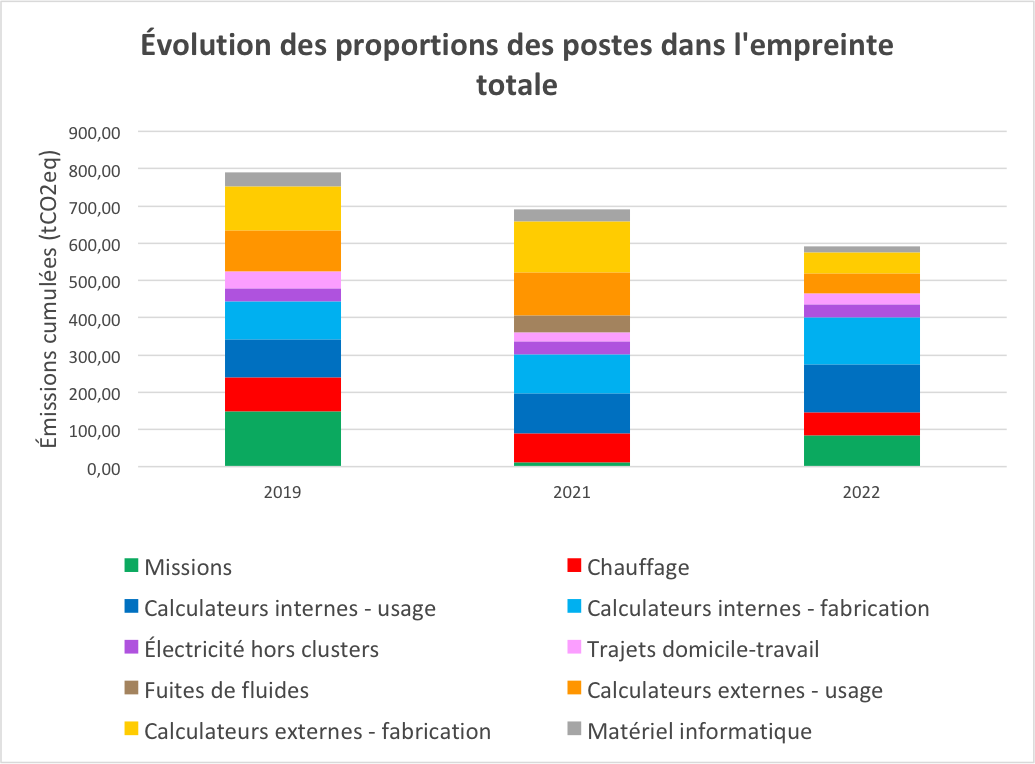
\includegraphics[width=0.85\textwidth]{images/evolution_postes_empreintecarbone.png}
    %    \caption{Évolution de l'empreinte carbone du CERFACS entre 2019 et 2022}
    %    \label{fig:evolution_empreinte_carbone}
    %\end{figure}

    Dans les couloirs du CERFACS, on trouve des posters très clairs sur l'empreinte carbone d'un trajet pour une conférence en fonction des moyens de transport.
    Les employés sont incités à venir à vélo. Le CERFACS donne une prime pour chaque kilomètre fait à vélo sur le trajet domicile-travail. Il y a aussi un atelier de réparation et des emplacements sécurisés pour les vélos.
    La politique de communication n'est pas spécialement tournée vers les efforts pour le climat ou la RSE, mais le CERFACS agit efficacement en ce sens.

\paragraph{Responsabilité sociale / Qualité de vie au travail}
    \begin{quote}
        \setlength{\leftmargin}{0.5cm} % Ajuster la marge gauche
        \setlength{\rightmargin}{0.5cm} % Ajuster la marge droite
        "La démarche Qualité de Vie au Travail (QVT) a été lancée au Cerfacs en janvier 2022, avec la mise en
        place d’un Groupe de Travail : elle a permis d’identifier 6 axes de travail pour améliorer le
        fonctionnement de la structure et du ressenti des personnes :
        \begin{itemize}
            \item Optimiser l’organisation et gestion du travail au niveau global
            \item Optimiser l’organisation et gestion du travail au niveau de l’équipe
            \item Optimiser l’organisation et gestion du travail au niveau personnel
            \item Assurer un meilleur accueil et support des non permanents
            \item Favoriser la vie sociale
            \item Améliorer le confort matériel"
        \end{itemize}
    \end{quote}

    %De nouveau, un tableau \annexref{tab:QVT_actions} détaille des exemples d'actions que j'ai pu expérimenter (salle de repos, machine à café, parking vélo, etc.).

    Un dernier plan d'action a été mis en place sur l'égalité professionnelle entre les femmes et les hommes. Il traite de divers sujets : l’embauche, la rémunération effective, l’articulation entre l’activité professionnelle et l’exercice de la responsabilité familiale.

    Je tiens à mentionner également que j'ai reçu un mail qui lançait un appel au volontariat pour composer le Comité de Pilotage pour la Prévention des Violences Sexistes et Sexuelles au Travail suite à une réunion d'information réalisée en collaboration avec la médecine du travail.

\newpage


Mon ressenti personnel sur le cadre de travail est très positif. Être assis dans un bureau climatisé avec une vue sur la campagne participe évidemment à cela. Un des seuls risques à ce type de travail est une mauvaise position qui peut entraîner des troubles musculosquelettiques. Pour pallier cela, il y a des affiches dans chaque bureau indiquant la meilleure position à avoir et proposant des exercices. Ces mêmes informations apparaissent dans le 'livret d'accueil stagiaire' qui m'a été remis le premier jour.
Une cantine présente sur le site à quelques minutes à pied, permet de déjeuner et échanger avec les collègues du CERFACS hors cadre professionnel.
\newpage

\chapter{Optimizing the performance of a centrifugal pump by data assimilation}



%En combien de temps l'information de pression remonte-t-elle dans le diffuseur ?


%144 coeurs : 54it/min
%300-> 336 coeurs : 100it/min (+- 20\%)

%– Le récit de l’expérience préprofessionnelle doit faire état de toutes les fonctions exercées par le stagiaire à son poste. Il doit comporter des développements techniques (illustrés par des schémas expliqués et commentés, par exemple), mais il s’agit avant tout de donner au lecteur une idée de ce que furent l’emploi du temps du stagiaire, ses tâches quotidiennes, les contraintes du métier, la nature des relations humaines dans cet environnement, les difficultés rencontrées et les résultats obtenus.
%– Les connaissances techniques acquises doivent transparaître dans le document. Le correcteur évaluera si celui-ci fait état d’une maîtrise réelle des outils (informatiques, mécaniques, etc.) utilisés pendant le stage. En outre, il estimera le niveau des connaissances techniques acquises que la rédaction du rapport aura su mettre en évidence.

The internship began in February 2025. I was provided with a fix computer, and credentials to connect to the Irene and Cassiopée supercomputers. Marcello MELDI, Antoine DAZIN and Miguel MARTINEZ VALERO which are my internship supervisors, showed me around the lab.
Then, Tom MOUSSIE and Miguel, my co-officies, explained to me the basics of OpenFoam and CONES, the DA code. I was able to run a few tests on OpenFoam on the supercomputers, which allowed me to familiarize myself with the tools and the code. % PARLER DE LA CONFIG DE CONES


% Introduction par thèse de Miguel

%Lors de mes essais sur le supercalculateur, j'ai utilisé une partition qui offre une puissance de calcul totale de 723 Tflop/s. Elle est composée de 185 nœuds Intel 2x18 cœurs Skylake, cadencés à 2,3 GHz avec 96 Go de mémoire. Ces ressources m'ont permis d'effectuer les tests demandant le plus de ressources.

\section{Data Assimilation}

% PAS d'equation ici, sinon je me fait frapper

DA\cite{aschDataAssimilationMethods2016} is a technique used to improve the accuracy of numerical models by combining them with observational data. It is widely used in various fields, including meteorology, oceanography, and engineering. The goal of data assimilation is to obtain a more accurate representation of the state of a system by integrating information from different physical measurements or hight fidelity sources. An illustration of the data assimilation process is shown in Figure \ref{fig:DAmap}.

% changer l'endroit de la citation

\begin{figure}[H]
    \centering
    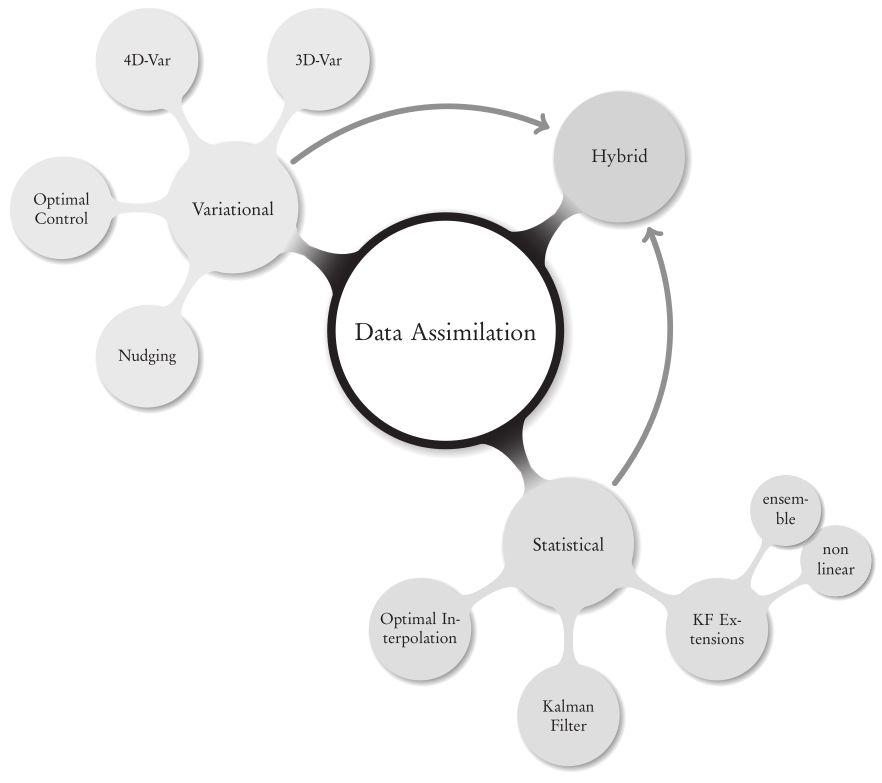
\includegraphics[width=0.60\textwidth]{images/other/DAmap.png}
    \caption{The big picture for DA methods and algorithms\cite{aschDataAssimilationMethods2016}}
    \label{fig:DAmap}
\end{figure}


\begin{figure}[H]
    \centering
    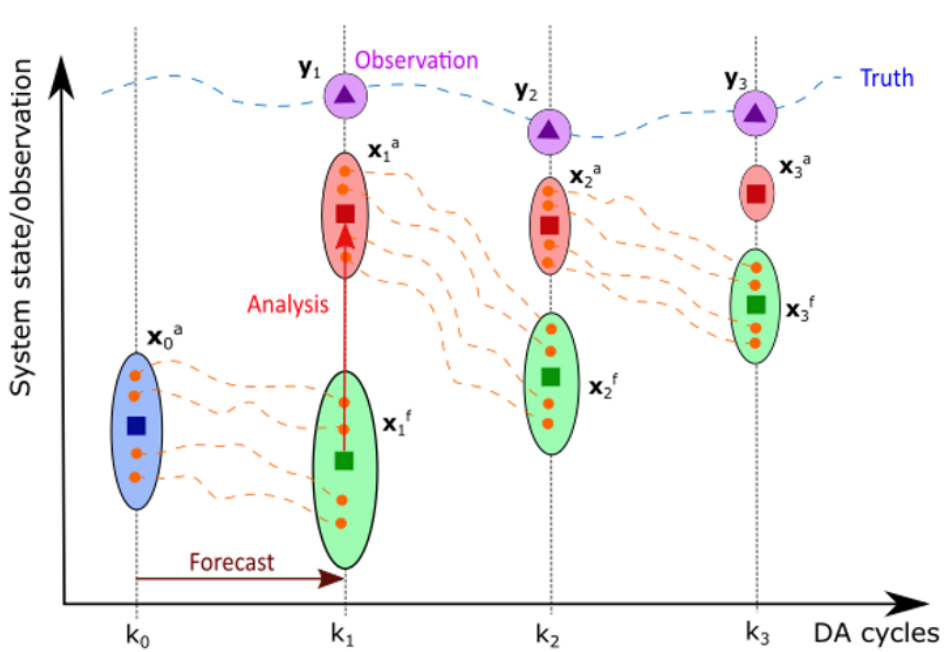
\includegraphics[width=0.60\textwidth]{images/enkf_shem.png}
    \caption{Illustration of the EnKF process (100\% confidence in observations)}
    \label{fig:EnKFIllustration}
\end{figure}


// Expliquer  théorème de Bayes etc... dans la partie maths (à ref ici)
%Expliquer plus en détail l'EnKF avec la fameuse figure.



\subsection{State of the art} % Introduction

\paragraph{EnKF} Our approach to data assimilation is based on the \ac{EnKF}, which is a Monte Carlo method that uses a set of model states (the ensemble) to estimate the state of the system. The EnKF is particularly well-suited for nonlinear systems and has been successfully applied in various fields, including computational fluid dynamics (CFD).

EnKF for DA in CFD has been used at LMFL since a few years, with the work of Lucas Villanueva\cite{villanuevaAugmentedStateEstimation2023}, Miguel M.Valero\cite{villanuevaAugmentedStateEstimation2023}, Tom Moussie\cite{moussieStatisticalInferenceUpstream2024a}, Sarp Er, Paolo Errante\cite{moussieStatisticalInferenceUpstream2024a} and Marcello Meldi\cite{villanuevaAugmentedStateEstimation2023}\cite{moussieStatisticalInferenceUpstream2024a} and his colleagues. The EnKF method is a powerful tool for assimilating data into computational fluid dynamics (CFD) simulations, allowing for the correction of model predictions based on observed data.



Today, we can theorically run a \ac{DNS} which resolves exactly the Navier-Stokes equations, but it is still too expensive to be used in practice. Therefore, we use \ac{LES} or \ac{RANS} models to simulate the flow. The EnKF method can be applied to these models to improve some of theme parameters or physical state, to improve the physical accuracy.

A good example based on the simple and academic \textit{cavity test case} illustrate it well.
The cavity test case is a simple flow in a square cavity, where the flow is driven by a moving lid. The flow is characterized by a recirculation zone and a vortex in the center of the cavity. The EnKF method can be used to assimilate data from the flow, such as velocity or pressure measurements, to improve the accuracy of the simulation. The EnKF method can also be used to estimate the parameters of the model, such as the viscosity or the turbulence model coefficients, to improve the physical accuracy of the simulation.
In our case, we are going to optimise the velocity wall condition.
For that, we use the result on 5 locations of a precise converged simulation with a to boundary condition of 5 m.s$^{-1}$ as a reference. We will then assimilate data from the flow, at the 5 observation points\ref{fig:cavity2_1ms}.
We start from a simulation with a wall condition of 1 m.s$^{-1}$, which is not the correct value. The EnKF method will then be used to correct the wall condition by assimilating the data from the flow at the 5 observation points. The EnKF method will iteratively update the wall condition until it converges to the correct value, which is 5 m.s$^{-1}$ in this case.

\begin{figure}[H]
    \centering
    \begin{subfigure}[b]{0.3\textwidth}
        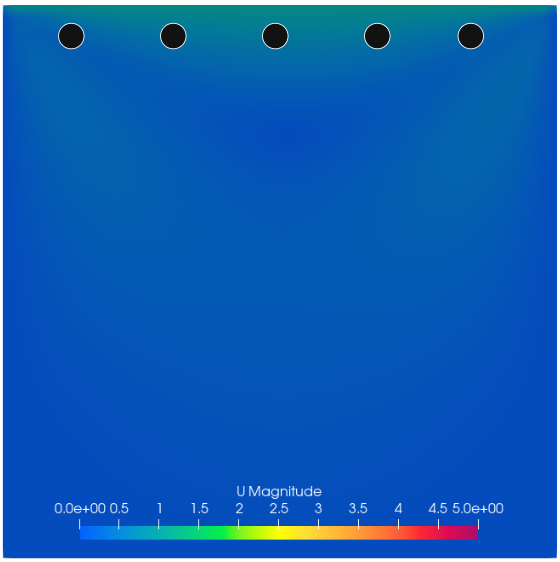
\includegraphics[width=\textwidth]{images/cavity/cavity3_1ms.png}
        \caption{Initial state}
        \label{fig:cavity2_1ms}
    \end{subfigure}
    \hfill
    \begin{subfigure}[b]{0.3\textwidth}
        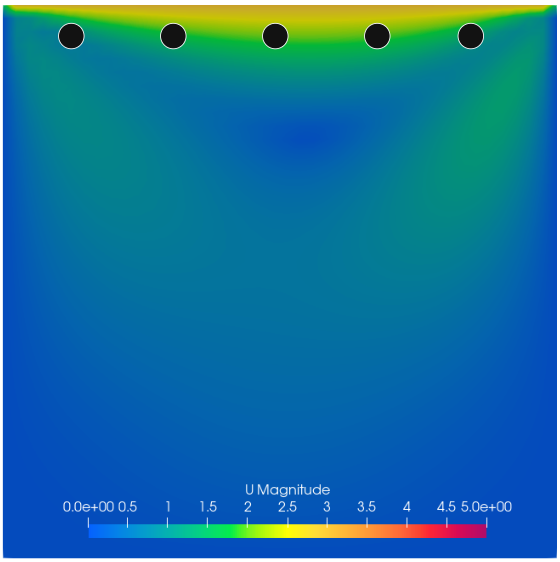
\includegraphics[width=\textwidth]{images/cavity/cavity3_3ms.png}
        \caption{After one EnKF it.}
        \label{fig:cavity2_3ms}
    \end{subfigure}
    \hfill
    \begin{subfigure}[b]{0.3\textwidth}
        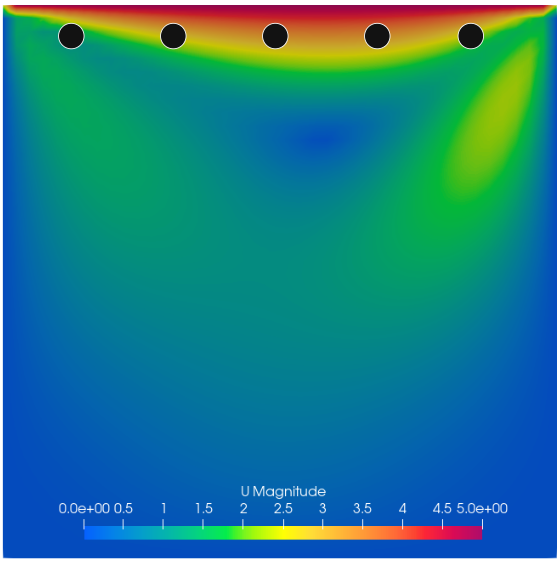
\includegraphics[width=\textwidth]{images/cavity/cavity3_5ms.png}
        \caption{Converged after 2 EnKF it.}
        \label{fig:cavity_5ms}
    \end{subfigure}
    \caption{Evolution of the state through EnKF iterations (
\includegraphics[width=0.014\textwidth]{images/cavity/legende.png}: observation point)}
\end{figure}




% Je cherche à transmettre quelle idée ?
% State of art : ce qui a été fait avant, ce qui est fait aujourd'hui, ce qui est fait dans le cadre de mon stage




\paragraph{IBM} The IBM theory has been developed in 1972 by Charles S. Peskin\cite{IBM_base}.
The Immersed Boundary Method (IBM) is a numerical technique used to simulate fluid-structure interactions, particularly in cases where the structure is immersed in a fluid flow. It permit to keep numerical precision on complex geometries and moving boundaries without the need for body-fitted meshes, which can be computationally expensive and difficult to implement.

They are differents ways to discretize the space when we do CFD (see Figure \ref{fig:solidworksMesh}\footnote{\url{https://www.solidworks.com/sw/docs/flow_basis_of_cad_embedded_cfd_whitepaper.pdf}}). The most common are structured meshes, unstructured meshes and body-fitted meshes. The body-fitted meshes are the most accurate but also the most expensive in terms of computational resources. The IBM allows to use unstructured meshes, which are less accurate but more efficient in terms of computational resources.

\begin{figure}[H]
    \centering
    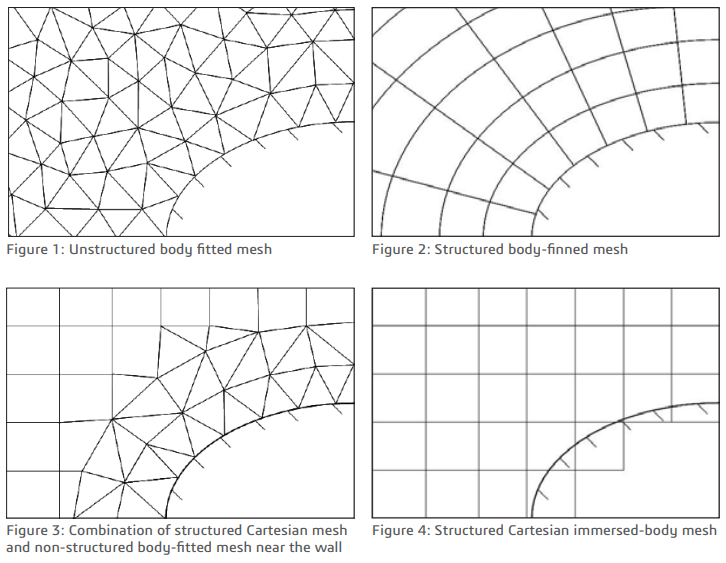
\includegraphics[width=0.8\textwidth]{images/solidworksMesh.png}
    \caption{Differents ways to mesh}
    \label{fig:solidworksMesh}
\end{figure}


In our case, we impose a forcing term on the Navier-Stokes equations to simulate the effect of the immersed boundary on the fluid flow. // ref à plus tard. The problem is that it it lead to a few constants that need to be tuned to obtain the best results. For that, we use the EnKF method to optimize these constants. The EnKF method will be used to assimilate data from the flow at the observation points and to update the forcing term until it converges to the optimal value.

These high fidelity data are obtained from an experiment explained in the next subsection
\begin{figure}[H]
    \centering
    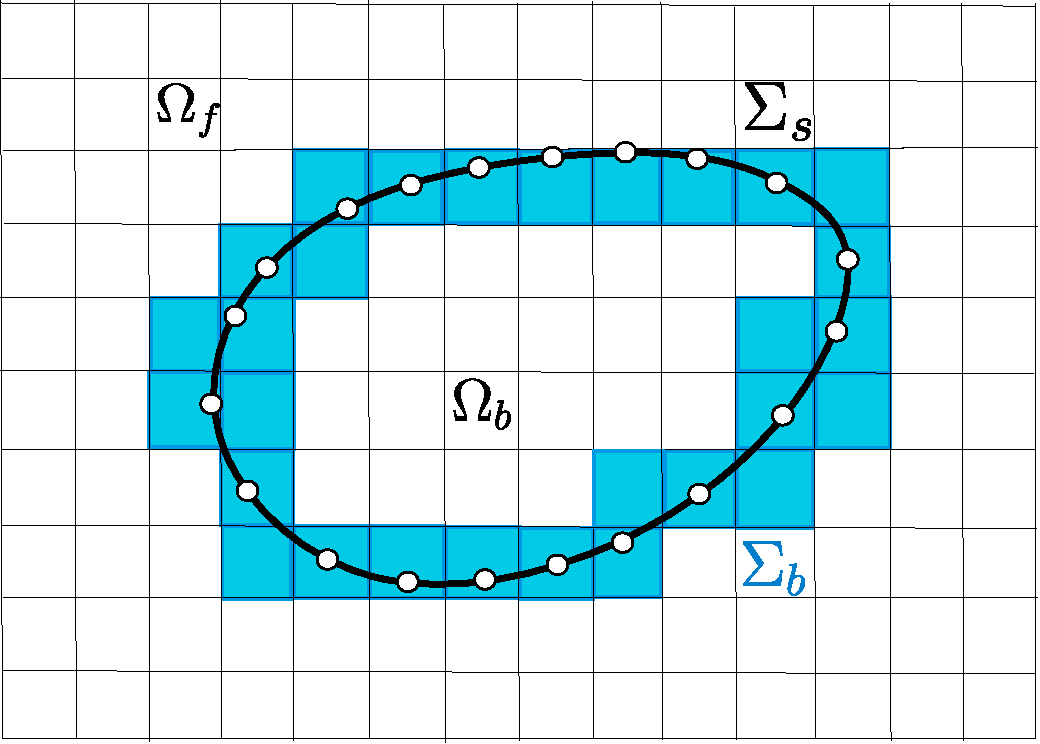
\includegraphics[width=0.45\textwidth]{images/IBM_Mesh.pdf}
    \caption{...}
    \label{fig:IBM_Mesh}
\end{figure}
Quel niveau de détail ici ?

% DONE (aller de + en plus en détail jusqu'a param IBM car gros cas test couteux en body-fitted)

This year, my supervisors M. VELRO and M. Meldi published an article\cite{valero2025immersed} about the optimisation of the IBM forcing and turbulence terms, that gives very good results. More recently, they obtain very good results on the optimisation of this parameters on a ascillating cylinder. // Tt ça à vérifier en relisant la thèse de Miguel.

% DONE Et là cas tests de thèse miguel (1 et 2)

This lead us to the idea of using the EnKF method to optimize the parameters of the IBM forcing term on a centrifugal pump, which is a more complex case than the previous ones. The goal is to improve the performance of the pump by optimizing the parameters of the IBM forcing term, which will lead to a better simulation of the fluid flow and a better understanding of the pump's behaviour.

% Puis amener cas 3 (pompe) pour transitionnre vers la sous-parite suivante

\subsection{Presentation of the test case: the centrifugal pump}


Parler rapidement qu'on a des données (pression et PIV)

Centrifugal pumps are used since 1475\cite{retiFrancescoDiGiorgio1963} and are still widely used today in various applications, such as water supply, irrigation, turbomachines, and industrial processes. They are known for their low cost, efficiency and reliability, making them a popular choice for many fluid transport applications.

\begin{figure}[H]
    \centering
    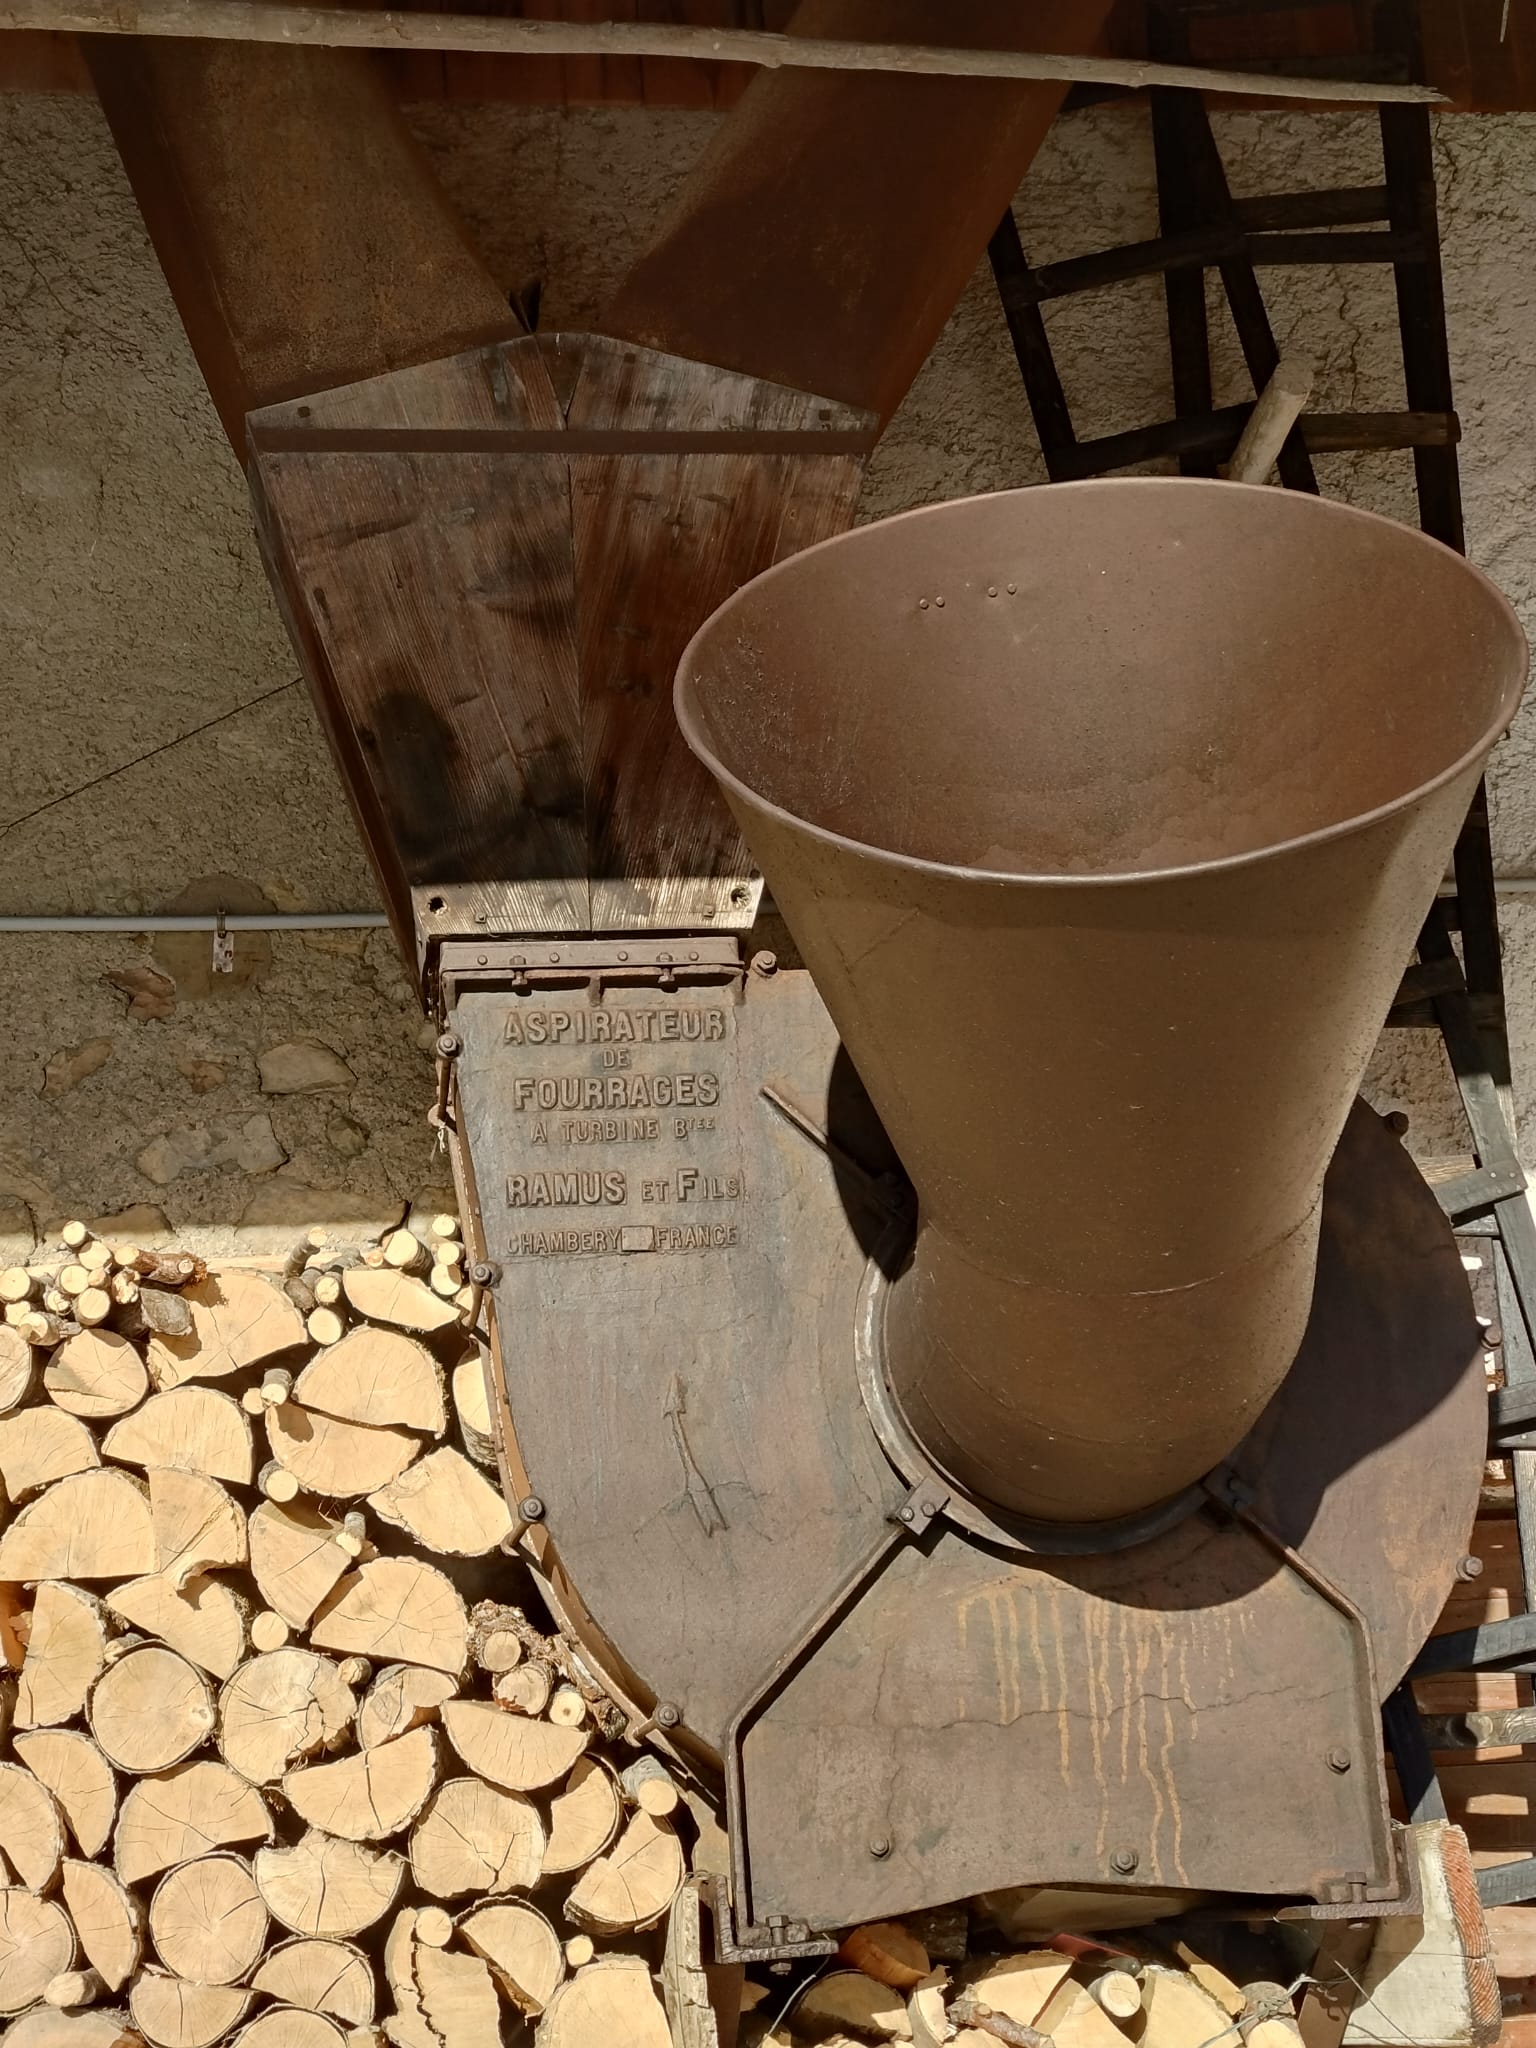
\includegraphics[width=0.40\textwidth]{images/other/pompe_centrifuge.jpg}
    \caption{Old centrifugal pump used to move hay (personnal picture)}
    \label{fig:old_centrifugal_pump}
\end{figure}


The studied centrifugal pump is a SHF impeller, which is a type of centrifugal pump designed for high flow rates and low head applications.
These high fidelity data are obtained from an experiment realised by Antoine Dazin\cite{dazinHighspeedStereoscopicPIV2011a} in 2011 at the LMFL. The experiment was realised on the SHF impeller on the RESEDA centrifugal pump benchmark. -> a vérifier dans la thèse de Miguel
% PARLER

Results in the file are High-Speed \ac{PIV} data obtained by Antoine DAZIN in 2011\cite{dazinHighspeedStereoscopicPIV2011a} at a PIV frequency of 980 Hz on a SHF impeller % Expliquer la PIV ?
The operating conditions of the machine where :

\begin{table}[!h]
    \centering
    \begin{tabular}{c c c}
        \multicolumn{3}{c}{\textbf{Impeller characteristics}} \\ \hline 
         $R_1$ & Tip inlet radius & $141.1\,mm$  \\
         $R_2$ & Outlet radius & $257.5\,mm$ \\ 
         $Z$ & Number of blades & $7$ \\
         $Q_d$ & Design flow rate & $0.236\,m^3/s$ \\ % 0.256 ???
         $K$ & Mean blade thickness & $9\,mm$ \\
         $\Omega$ & Rotating velocity & $1\,200\,rpm$ \\ 
         $\beta_2$ & Outside blade angle (from peripheral velocity $U=R_2\Omega$) & $22.5^{\circ}$ \\ \hline \hline
        \multicolumn{3}{c}{\textbf{Vaneless diffuser characteristics}} \\ \hline
         $b_3$ & Diffuser width & $38.5\,mm$ \\
         $R_3$ & Inlet radius (without leakage, i.e., $R_3=R_2$) & $257.5\,mm$ \\
         $R_4$ & Diffuser outlet radius & $385.5\,mm$ \\
         $t$ & Thickness of the upper and lower sections of the diffuser & $20\,mm$
    \end{tabular}
    \caption{Summary of the main geometrical and operating parameters of the impeller and diffuser at design conditions, employed in the numerical modelling of the centrifugal pump.}
    \label{tab:pump_parameters}
\end{table}


\begin{figure}[H]
    \centering
    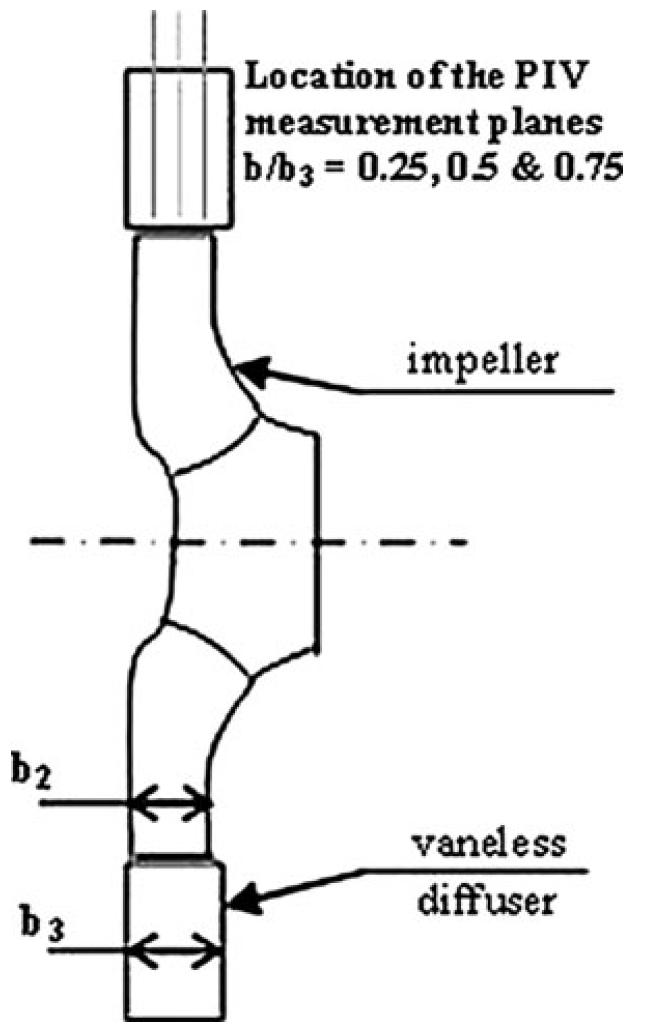
\includegraphics[width=0.4\textwidth]{images/experimentalPump/impeller_position.png}
    \caption{Position of the PIV plans}
    \label{fig:PIVPlans}
\end{figure}

The data is stored in a directory structure that contains 6 directories
The 6 directories are corresponding to two tests realised at 25\%, 50\% et 75\% of the diffuser height.
Each test was repeated twice for the same operating condition and the same height (R1, R2)
In each directory, there are 1581 files corresponding to instantaneous ASCII data file.
The 9 columns are corrresponding to :

%centrer
$x(m),y(m),V_x(m.s^{-1}),V_y(m.s^{-1}),r(m),\theta(rad),Vr(m.s^{-1}),V_{\theta}(m.s^{-1}),V_z(m.s^{-1}),\textit{Unknown}$

%The pdf is a paper where can be found the experimental conditions even if the analysis are focussed on another flow rate.

The theorical average speed at the input of the diffuseur is equal to \[\frac{Q_{dif_{in}}}{S_{dif_{in}}} = \frac{Q_{pump_{in}}}{2\pi R_{3} h_{dif}} = 3.65m.s^{-1}\]
With $Q_{pump_{in}} = Q_{dif_{in}}$ because the mass flow rate is constant and the flow is incompressible.

%Détail : R3 = 0.257m; h=0.0400m; Q = 0.236m3/s -> S=0.0646m2

\title{Fonctionning}  % ????
\title{Utility}


%Données hautes fidélités,...


\section{Numerical ingredients}

\subsection{CFD governing equations}



\begin{equation}
    (\boldsymbol{u} \cdot \boldsymbol{\nabla})\, \boldsymbol{u} = 
    -\frac{1}{\rho} \nabla p + \nu \nabla^2 \boldsymbol{u} 
    \underbrace{- \xi \nu \boldsymbol{D} \left( \boldsymbol{u} - \boldsymbol{u}_{ib} \right)}_{\boldsymbol{f}_P}
\end{equation}



with $[p] = M \cdot L^{-1} \cdot T^{-2}$ 
(formalisme divisé par la masse volumique $\rho$. Donc $[\boldsymbol{u}] = L \cdot T^{-1}$ - en incompressible).

\begin{equation}
    \xi = \left\{
    \begin{array}{ll}
        0 & \textrm{if } \boldsymbol{x} \in \Omega_f \\
        1 & \textrm{if } \boldsymbol{x} \in (\Sigma_b \cup \Omega_b)
    \end{array} \right.
\end{equation}

see Figure \ref{fig:IBM_Mesh}

When  $D \rightarrow \infty$, problèmes
        
mais des valeurs trop élevées de $D$ peut mener à des instabilités <- A mentionner qqpart 




Fluid mechanics is governed by the NS equations :




- Equations (Incompressible, turbulence,...)
- Ajout IBM\ref{fig:IBM_Mesh} -> Methodo (forcage continue ici (vs interpolation ?)) -> avantages
- Ajout MRF

% A écrire à ma facon, juste équations intéréssantes ici
Darcy's law in the body interface region $\Sigma_b$ and the solid region $\Omega_b$. To do so, a spatial dependent tensor $\boldsymbol{D}(\boldsymbol{x})$ must be defined. The resulting penalty term is modelled as follows:

\begin{equation}
     \boldsymbol{f}_P = \left\{
        \begin{array}{ll}
        \boldsymbol{0} & \textrm{if } \boldsymbol{x} \in \Omega_f \\
        -\nu \, \boldsymbol{D} \left(\boldsymbol{u} - \boldsymbol{u_{ib}} \right) & \textrm{if } \boldsymbol{x} \in (\Sigma_b \cup \Omega_b)
        \end{array} \right.
    \label{eqn:forcePenDarcy}
\end{equation}
$\boldsymbol{u_{ib}}(\boldsymbol{x}, t)$ is a target velocity representing the immersed body's physical behaviour. ... $\boldsymbol{u_{ib}}=\boldsymbol{0}$. The components $D_{ij}$ of the tensor $\boldsymbol{D}$ are usually controlled to obtain the best compromise between the accuracy and stability of the numerical solver %\cite{Verzicco2022_arfm}. The choice performed is crucial in the proximity of the grid transition between the fluid $\Omega_f$ and the interface $\Sigma_b$ regions.

$Re_\Omega=\cfrac{R_2^2 \Omega}{\nu} = 5.53\times10^5$ 

$Ma = \cfrac{R_2 \Omega}{c} = 0.095$ \textrm{\textbf{(incompressible)}}

Reprendre ma présentation (dimensiosn de p)

\begin{equation*}
    \boldsymbol{\nabla} \cdot (\boldsymbol{u}\boldsymbol{u}) = -\nabla p + \nu \nabla^2 \boldsymbol{u}  \overbrace{-\frac{\xi}{\eta} \left(\boldsymbol{u} - \boldsymbol{u_{ib}} \right)}^{\boldsymbol{f}_P}
\end{equation*}

\begin{equation*}
    \xi = \left\{
   \begin{array}{ll}
   0 & \textrm{if } \boldsymbol{x} \in \Omega_f \\
   1 & \textrm{if } \boldsymbol{x} \in (\Sigma_b \cup \Omega_b)
   \end{array} \right.
\end{equation*}

\subsection{The open source code OpenFoam}

To implemente the IBM forcage, we use the open source code OpenFoam, which is a C++ library for computational fluid dynamics (CFD). OpenFoam provides a wide range of tools for solving the Navier-Stokes equations, including solvers, meshing tools, and post-processing tools. It is widely used in the CFD community and has a large user base.

More precisely, for example, to implemente the IBM forcage on the speed U, we compute the forcing term $\boldsymbol{f}_P$ as follows:
\begin{lstlisting}[language=C++]
// Compute the forcing term
volVectorField fP = -fP_ * (U - U_ib); EXEMPLE DE MISE EN FORME A CORRIGER
// Add the forcing term to the momentum equation
U += fP;
\end{lstlisting}

\begin{figure}[H]
    \centering
    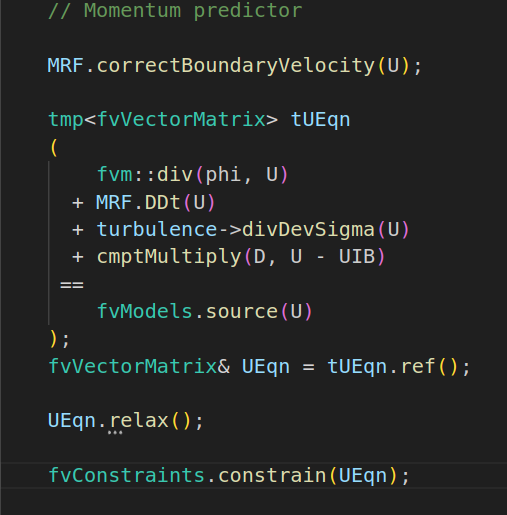
\includegraphics[width=0.5\textwidth]{images/other/implicit_forcing.png}
    \caption{implicit forcing term in OpenFoam}
    \label{implicit_forcing}
\end{figure}




To compute the time step $\Delta_{t}$ of the pimpleFoam simulation of the pump, we can use the \ac{CFL} condition, which states that:
\begin{equation}
    \Delta_{t} = \frac{CFL \cdot \Delta_{x}}{\|U_{\infty}\|},
\end{equation}
where:

- $CFL$ is the Courant number, typically set to 0.5 for stability. A way to visualize this is to think of it as the fraction of the distance a wave travels in one time step relative to the distance between two cells in the azimuthal direction at the tip of the impeller.
- $\Delta_{x}$ is the distance between two cells in the azimuthal direction at the tip of the impeller in our model, which is given as 1.5 mm or 0.0015 m.
- $\|U_{\infty}\|$ is the magnitude of the velocity at infinity, which can be approximated by the tangential velocity at the tip of the impeller.
\begin{equation}
    \|U_{\infty}\| = \omega \cdot r_{tip}
\end{equation}
where:
- $\omega$ is the angular velocity in radians per second,
- $r$ is the radius at the tip of the impeller.
Assuming the rotating speed is given in revolutions per minute (rpm), we can convert it to radians per second:
\begin{equation}
    \omega = \frac{1200 \text{ rpm} \cdot 2\pi \text{ rad}}{60 \text{ s}} = 125.66 \text{ rps}.
\end{equation}
Assuming the radius at the tip of the impeller is $r = 0.2566 \text{ m}$ (which is 0.2566m), we can compute the tangential velocity:
\begin{equation}
    \|U_{\infty}\| = 125.66 \text{ rps} \cdot 0.2566 \text{ m} =  \text{32.24 m/s}.
\end{equation}
Assuming the distance between two cells in the azimuthal direction at the tip of the impeller is $\Delta_{x} = 0.0015 \text{ m}$ (which is 1.5 mm), we can now compute the time step $\Delta_{t}$:
\begin{equation}
    \Delta_{t} = \frac{0.5 \cdot 0.0015 \text{ m}}{32.24 \text{ m/s}} = 2.3 \times 10^{-5} \text{ s} % \approx 2.3 \mu s.
\end{equation}


\subsection{EnKF}

Toujours mentionner les paramètres utilisés (dans le controlDict et le CONESDict)

\subsection{The library CONES}
CONES is a library coded in Python/C++ developed for ... since 2022 at LMFL. -> appuyer sur "seule online pour CFD à la connaissance du labo"
It's parallelized and can be used on supercomputers. It is mainly designed to work with OpenFoam and DA codes as EnKF.\label{instants_partages}

Simulations are performed using the C++ framework OpenFOAM, used to discretize the equations previously presented. Standing for \textsl{Open Source Field Operation and Manipulation}, OpenFOAM is an open-source which provides many tools, referred to as executables %\citep[see][]{greenshields2021}. These executable files can be divided into three separate categories:
\begin{itemize}
    \item[$-$] \textbf{Pre-processing}, including meshing and decomposing tools.
    \item[$-$] \textbf{Solving}, including in-built and custom solvers. Each solver is built to answer a specific CFD problem. 
    \item[$-$] \textbf{Post-processing}, including \texttt{ParaView}, an open-source visualization application.
\end{itemize}

OpenFOAM is not provided with a graphical interface, which is why a simulation is built by writing ``dictionaries'', in which are stored the necessary information for the simulation (mesh, turbulence model, maximum number of characteristic times, $\dots$). Thus, a specific directory structure must be observed, as outlined in ... % \autoref{fig:OpenFOAM_directory_structure}:
% décrire la structure du dossier OpenFOAM et ce que chaque fichier fait (dans mon cas de simulation)

\begin{figure}[H]
    \centering
    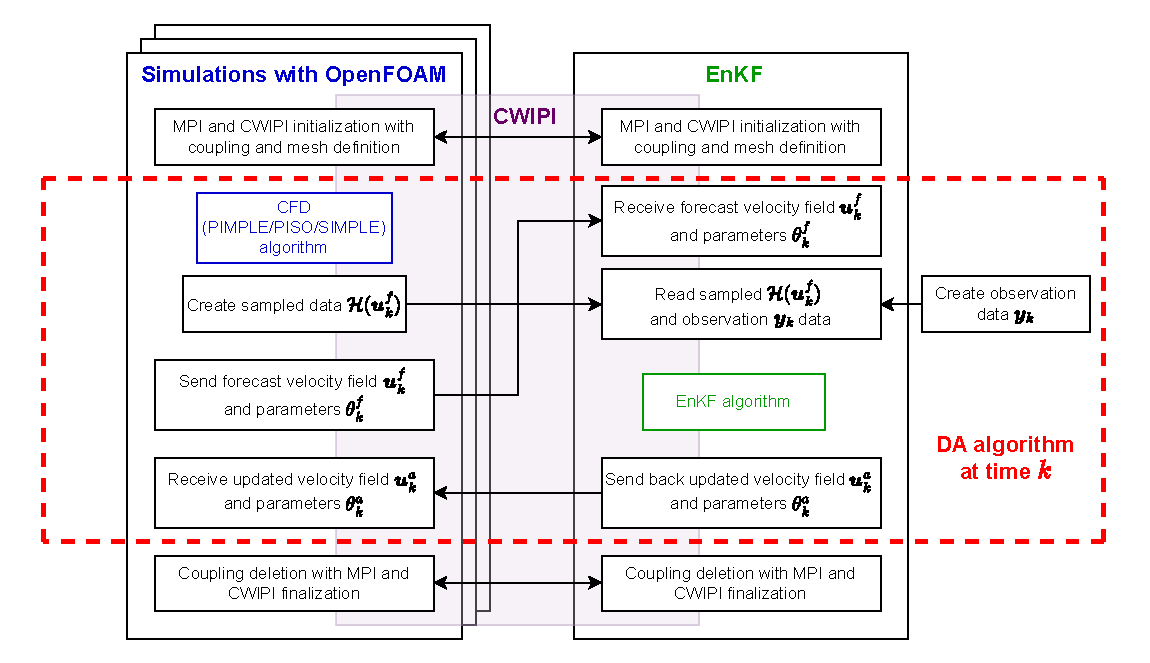
\includegraphics[width=0.5\textwidth]{images/EnKF_Cones.pdf}
    \caption{Model}
    \label{model}
\end{figure}


\begin{forest}
    for tree={
      font=\ttfamily,
      grow'=0,
      child anchor=west,
      parent anchor=south,
      anchor=west,
      calign=first,
      inner xsep=7pt,
      edge path={
        \noexpand\path [draw, \forestoption{edge}]
        (!u.south west) +(7.5pt,0) |- (.child anchor) pic {folder} \forestoption{edge label};
      },
      before typesetting nodes={
        if n=1
          {insert before={[,phantom]}}
          {}
      },
      fit=band,
      before computing xy={l=15pt},
    }  
  [root
    [system
      [controlDict
      ]
      [blockMeshDict
      ]
      [decomposeParDict
      ]
      [fvSchemes
      ]
      [fvSolution
      ]
    ]
    [templates
    ]
    [tests
    ]
  ]
  \end{forest}



\begin{figure}[H]
    \centering
    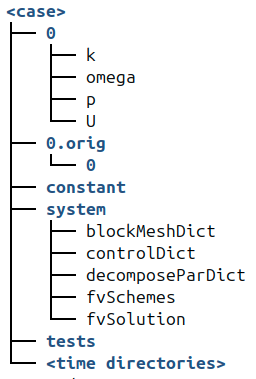
\includegraphics[width=0.3\textwidth]{images/other/OF_arbo.png}
    \caption{Arbo of OpenFoam}
    \label{arboOF}
\end{figure}


The \texttt{system} directory contains the main parameters concerning the progress of the simulation:
\begin{itemize}
    \item[$-$] The \texttt{controlDict} dictionary defines parameters such as start and end time, time steps, data output formatting, or data average computation.
    \item[$-$] The \texttt{blockMeshDict} dictionary defines the geometry, mesh and boundary conditions implementation.
    \item[$-$] The \texttt{decomposeParDict} dictionary defines the geometry and mesh decomposition, with the objective to run the simulation in parallel, using multiple cores.
    \item[$-$] The \texttt{fvSchemes} dictionary defines the discretisation schemes used in the solution.
    \item[$-$] The \texttt{fvSolution} dictionary defines the equation solvers, tolerances and other algorithm controls for instance. 
\end{itemize}

The \texttt{constant} directory contains the different physical properties of the simulation. Moreover, the subfolder \texttt{polyMesh} contains the mesh data, obtained after the \texttt{blockMesh} command line is run:
\begin{itemize}
    \item[$-$] The \texttt{momentumTransport} dictionary defines the simulation type (\ac{RANS} or \ac{LES}), as well as the turbulence model.
    \item[$-$] The \texttt{transportProperties} dictionary defines the transport model (Newtonian for instance) and some transport coefficients, such as the kinematic viscosity $\nu$. 
    \item[$-$] The \texttt{turbulenceProperties} dictionary defines the different parameters of the chosen turbulence model.
\end{itemize}

The \texttt{0} directory contains the initial solution's fields. The \texttt{postProcessing} directory stores data from the running simulation, such as forces and probes' data. The \texttt{processor0...N} directories directly result from the geometry decomposition, which is proceeded through the \texttt{decomposeParDict} dictionary. The \texttt{dummy.foam} is an empty file which allows to visualize the simulation with \texttt{ParaView}. 


\subsection{Pump modeling}

The objective of the model is to try to find same physical behavior as the experimental data. We call that digital twin.

For that we have first to discretize the numerical model of the pump. The mesh is generated using the \texttt{blockMesh} utility, which is a built-in OpenFOAM tool. The mesh is composed of 12 million cells. The mesh is composed of hexahedral cells. (quasi only, exepted some interface, cf figure). We don't need complex mesh because we dont neek to fit the geometry of the impeller.

Boundary conditions are defines as that:
\begin{itemize}
    \item[$-$] Inlet: velocity inlet
    \item[$-$] Outlet: pressure outlet
    \item[$-$] Wall: no-slip wall
\end{itemize}


\begin{figure}[H]
    \centering
    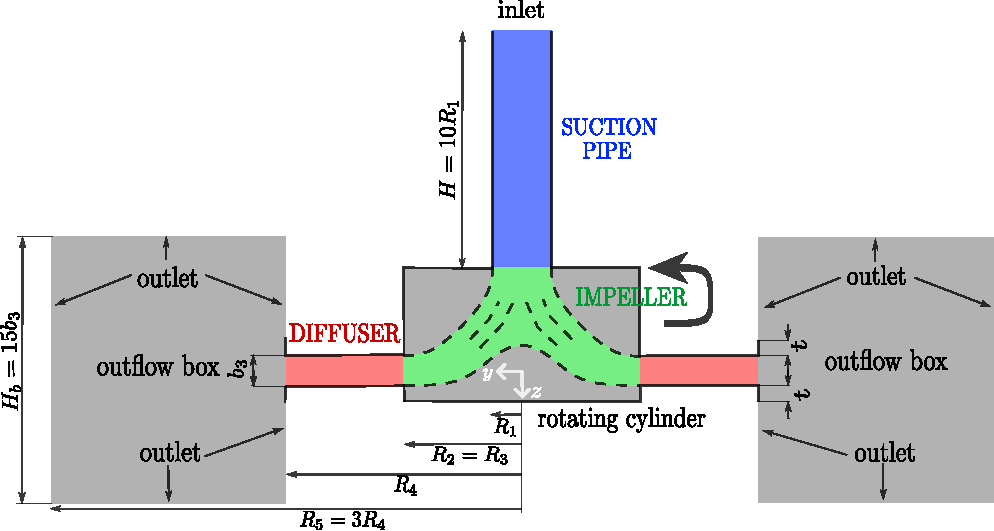
\includegraphics[width=0.5\textwidth]{images/model/RESEDA_sketch.pdf}
    \caption{Model}
    \label{Model}
\end{figure}

\section{IBM preliminary results}

"Résultats de la simulation avec 3e5" -> 3e7





Graçe aux données xp (mentionné partie 2.1.2, on peut faire d la DA)



\begin{figure}[H]
    \centering
    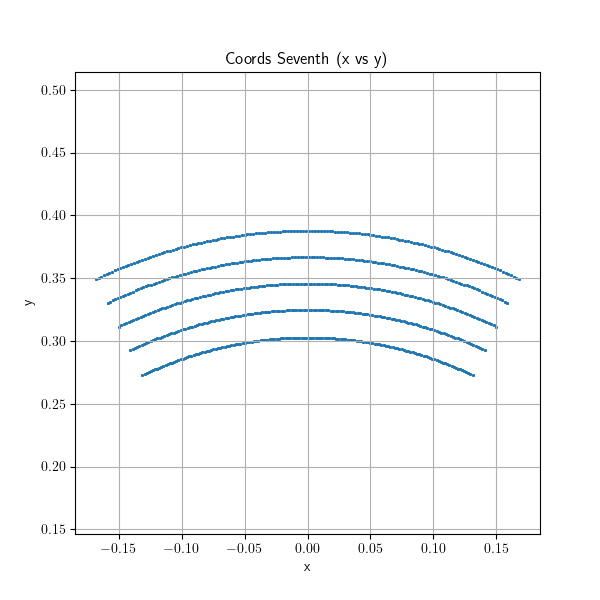
\includegraphics[width=0.5\textwidth]{images/coordsSeventh.png}
    \caption{Interpolation points over 360/7 degrees}
    \label{coordsSeventh}
\end{figure}


Notre but : faire fit ces 2 courbes : 

\begin{figure}[H]
    \centering
    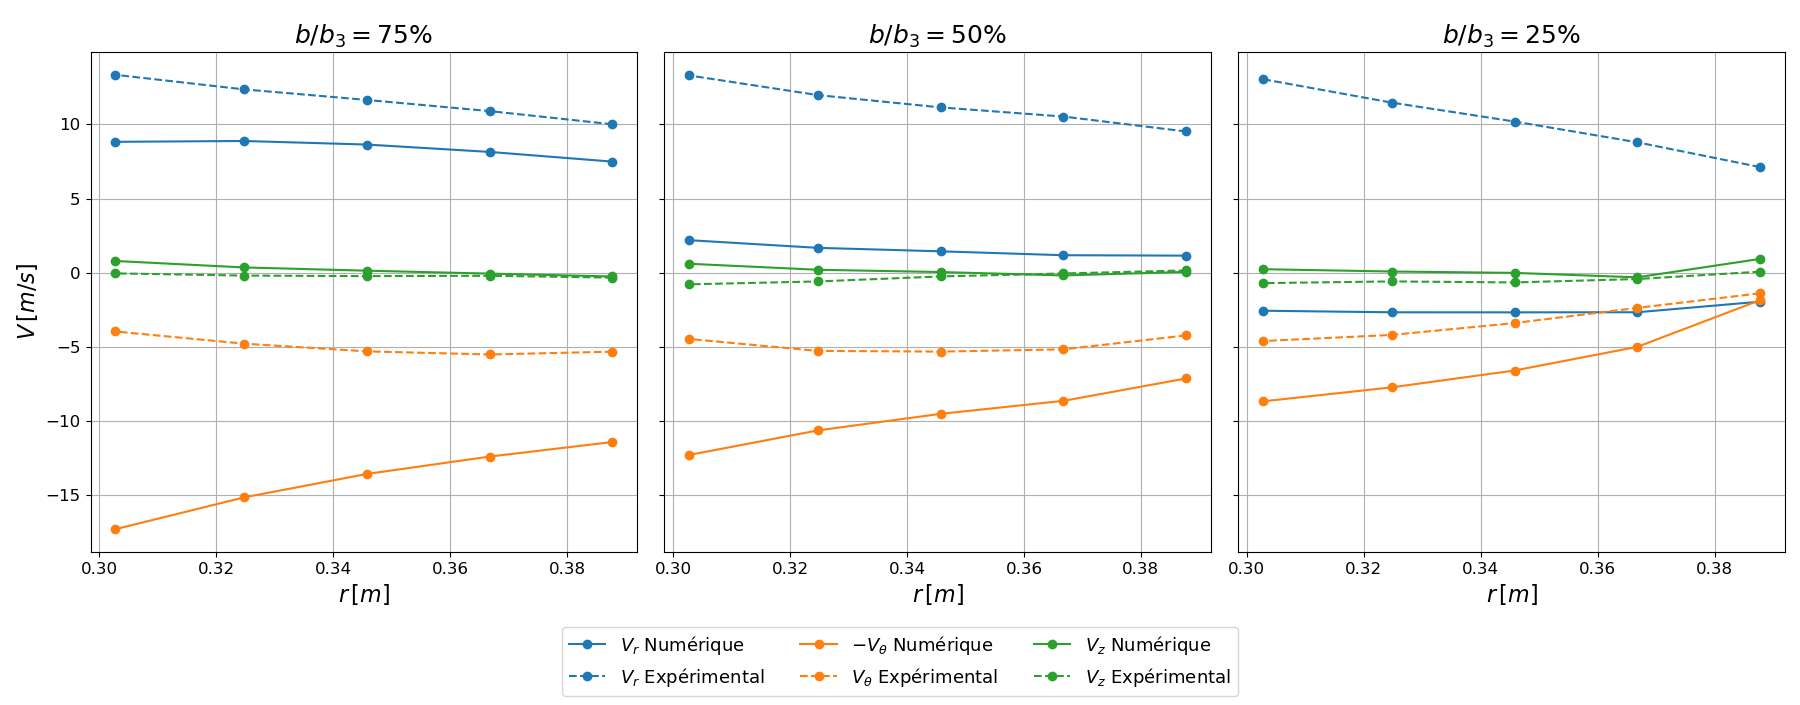
\includegraphics[width=1\textwidth]{images/numVSxp.png}
    \caption{implicit forcing term in OpenFoam}
    \label{numVSxp}
\end{figure}

Mais surtout obtenir le bon rendement ! (sujet du stage)

\begin{figure}[H]
    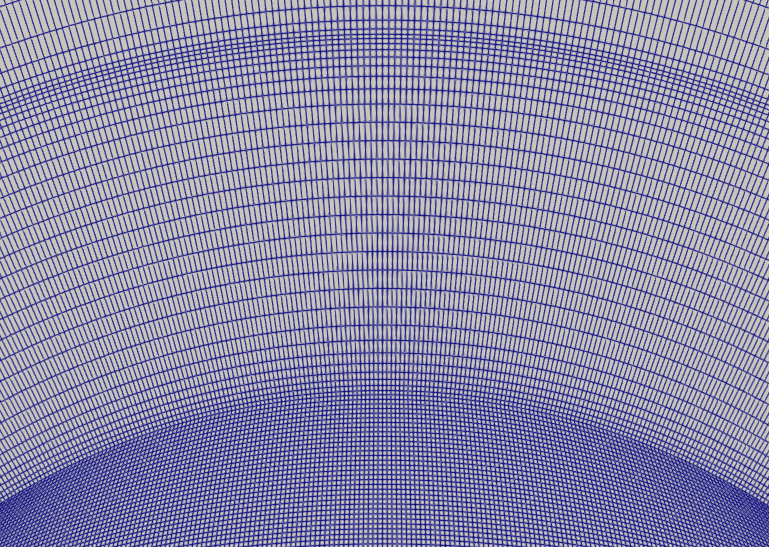
\includegraphics[width=0.4\textwidth]{images/numericalPump/diffuseurMesh.png}
    \caption{diffuseur Mesh}
    \label{diffuseurMesh}
\end{figure}

\begin{figure}[H]
    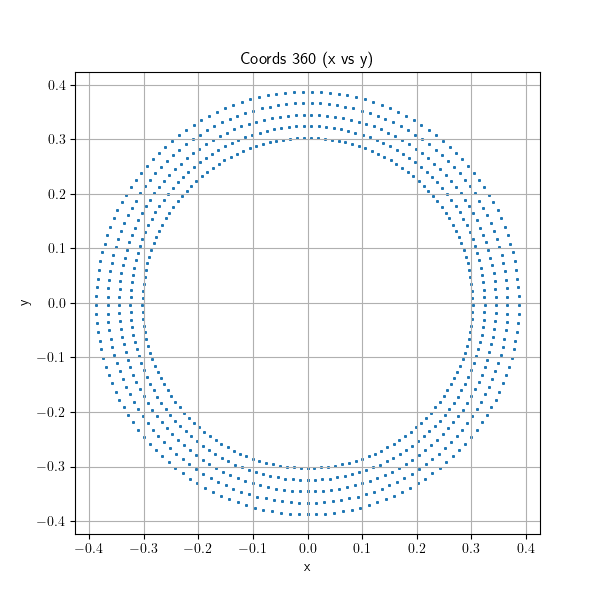
\includegraphics[width=0.4\textwidth]{images/coords360.png}
    \caption{Interpolation points over 360 degrees}
    \label{coords360}
\end{figure}

Limitations IBM à améliorer avec DA


\section{Application of the DA}

Explication de coords\_seventh.txt, coords\_360.txt et coords\_7.txt

Tentative d'explication en français :

J'ai d'un coté une simulation numérique de la pompe centrifuge, qui est un modèle numérique de la pompe. De l'autre coté, j'ai des données expérimentales de PIV, qui sont des données expérimentales de la pompe centrifuge. Je veux utiliser les données expérimentales pour améliorer le modèle numérique de la pompe centrifuge.
Pour cela, j'utilise la méthode de l'assimilation de données, qui est une méthode qui permet d'améliorer un modèle numérique en utilisant des données expérimentales. La méthode que j'utilise est l'Ensemble Kalman Filter (EnKF), qui est une méthode d'assimilation de données qui utilise un ensemble de modèles numériques pour améliorer le modèle numérique. 
Cela se fait en deux étapes :
\begin{enumerate}
    \item Je fais une simulation numérique de la pompe centrifuge, en utilisant le modèle numérique de la pompe centrifuge. Cette simulation numérique me donne un ensemble de modèles numériques, qui sont les membres de l'ensemble.
    \item Je compare les données expérimentales de PIV avec les données numériques de la simulation numérique. Pour cela, je fais une interpolation des données expérimentales de PIV sur les points de l'ensemble de modèles numériques. Cette interpolation me donne un ensemble de données expérimentales, qui sont les observations.
\end{enumerate}

La comparaison entre les données expérimentales et les données numériques me permet de calculer l'écart entre les deux, qui est appelé l'innovation (mettre référence partie mathématique). L'innovation est utilisée pour mettre à jour les membres de l'ensemble de modèles numériques, en utilisant la méthode de l'EnKF. Cette mise à jour me permet d'améliorer le modèle numérique de la pompe centrifuge.

1. Ma simulation numérique de la pompe est stationaire en utilisant la méthode MRF. Cela signifie que le champ de vitesse est constant dans le temps. Cepandant, il n'est pas constant dans l'espace, car il dépend de la position dans le diffuseur. Un motif de vitesse répété sept fois est donc censé être visible (cela n'est pas vraiment le cas en instantionnaire).

2. Les données PIV sont acquises à une vitesse de rotation de la pompe et une fréquence telle que 49 images sont acquises par tour de roue, soit 7 immages entre deux passage d'aubes successives. Dans le référentiel de la pompe, les images sont prises à un une différence de 360/49deg. 

Nous voulons comparer des données consitantes. Nous pourrions syncroniser une simulation instationnaire avec les données PIV. Mais nous avons choisis de faire une simulatio instationnaire dans un premier temps.

Nous pourrions reconstruire le champ spatial PIV (nous avons assez d'angle de vue et de données pour cale -> ref article Antoine).
Cependant, la vitesse de rotation n'est pas très précise, mais surtout, la méthode MRF inverse la forme du sillage.

Nous avons donc choisis de moyenner temporellement les données PIV (ce qui reviens à moyenner spatialement).
Du coté de la simulation, nous avons donc besoin de moyenner azimutalement les données numériques pour les rendre compatibles avec les données PIV.

\begin{figure}[H]
    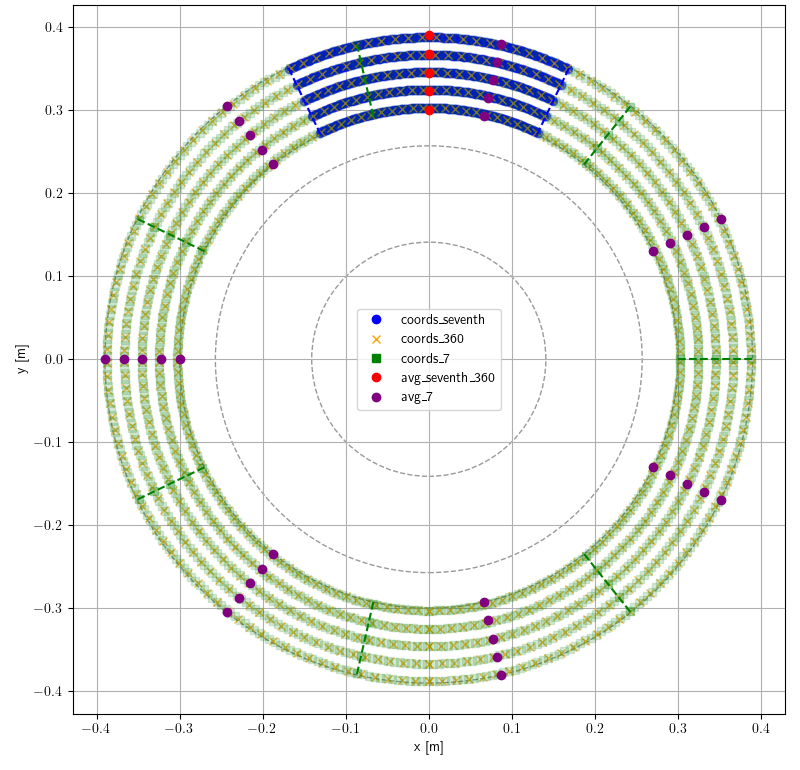
\includegraphics[width=0.8\textwidth]{images/numericalPump/coords.png}
    \caption{}
    \label{CHANGER}
\end{figure}

Imager avec des illustrations et vue en coupe ParaView

Pour cela j'ai commencé en moyennant 1/7 mais les paramètres étant locaux (non globaux), j'ai ensuite moyenné sur 360 degrés, ce qui permet de mieux prendre en compte les variations locales des paramètres. Cependant, nous pouvons converger vers une moyenne physique qui atteinds un minimum local mais qui ne respecte pas d'avoir 7 fois le même pattern. Cela permet à Fx d'être très différent de Fy mais aussi à la simulation de diverger avec des paramètres et vitesses erronéees. Pour palier ce problème, je compare la moyenne des patternes sur mes 7 segments de 360/7 degrés.





%S'aider du plan de la présentation MALEAF + thèse M

%Expliquer comment j'applique la DA sur le cas test de la pompe centrifuge (pas d'equation)

Nous avons fait l'EnKF sans l'état\dots
Sans inflation pour commencer. Si on converge vers une solution qui ne nous satisfait pas, on peut essayer d'ajouter... Cela permet de s'échaper d'un minimum local en ajoutant du bruit artificiellement. 

Nous avons fait une simu RANS mais nous aurion pu faire une simu URANS (ou LES ou DDES) avec un modèle de turbulence... 

L'expérience montre un ordre de grandeur de centaines d'itération entre les phases d'analyse, mais cela dépend beaucoup du cas.
Il en est de même pour le nombre de phases d'analyse.
Supposons 1000 itération en moyenne entre chaque phase d'analyse, et 300 phases d'analyse, cela nous fait 300 000 itérations à simuler, soit 93h, sur env. 2800 coeurs, soit 264kh.processeur de calcul.

Comment calculer la variance que je veux mettre ?
Expérience : 5\%
De mon coté : je vise qu'en moyenne un membre d'ensemble ait un écart de 1e7 par rapport au temps précédent (pour des valeurs autour de 5e7), donc, pour 30 membres d'ensemble, environ 95\% = 2 sigma dans 5e7+-1e7, càd sigma = 0.5e7 = 10\%. Ensuite, le nombre d'itération entre les phases d'analyse est déterminé en regardans combien d'itération sont nécessaires pour faire varier la solution dans le diffuseur (influe, rapidement, converge doucement mais ce qui nous intéresse c'est que ça prenne la tendace) lorsqu'un paramètre de forcage est modifié (supposé très inférieure pour la turbulence car appliquée de partout)

The observation window was defined by observing the number of iterations required for the influence of the IBM to reach the diffuser and take the form of the converged result. We are not interested in the turbulence parameters to determine the observation window because they are present throughout the domain, their influence is almost direct (not necessarily their convergence). We chose 800 iterations


Pb de la DA : plus rapide que DNS mais toujours plus lent que RANS et le temps d'attente et de calcul sur supercalculateur (sur 4000 processeurs) est de l'orde de plusieurs jours. On peut donc se demander si la DA est vraiment utile dans ce cas. En effet, la DA est plus rapide que la DNS mais pas que la RANS. Cependant, il faut prendre en compte le fait que la DA permet de réduire le temps de calcul de la simulation numérique en permettant d'optimiser les paramètres de l'IBM. De plus, la DA peut être utilisée pour d'autres cas d'étude où la DNS est trop coûteuse.



Pb perso : jusqu'à plusieurs jours d'attente pour lancer une simu.
%\begin{figure}[H]
%    \centering
%    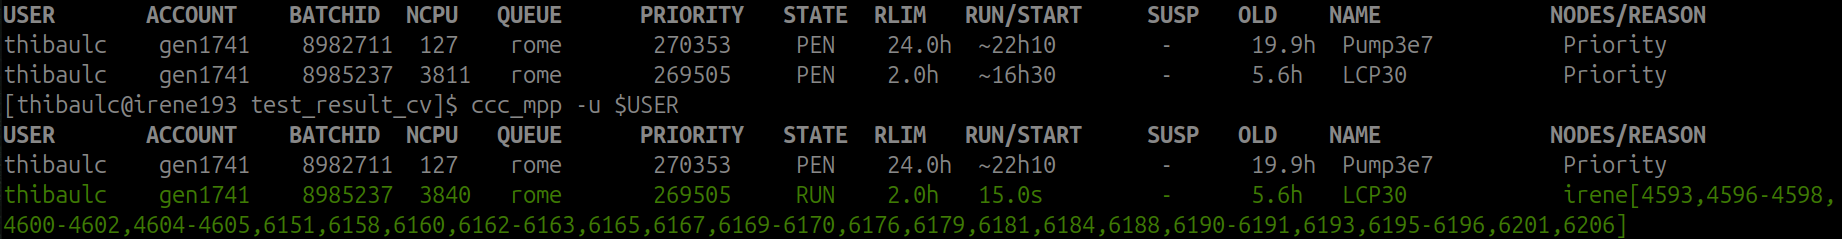
\includegraphics[width=0.5\textwidth]{images/other/queue_IRENE.png}
%    \caption{IRENE queue}
%    \label{queue_IRENE}
%\end{figure}

\subsection{Preprocessing of PIV data}

\subparagraph{Zone d'acquisition PIV}
\phantom{-}

The PIV data is acquired in a rectangular zone of 0.08 m x 0.124 m.
The cathesian coordinates are given in a local system, where the absolute origin is at the center of the pump.


\begin{figure}[H]
    \centering
    \begin{tikzpicture}
        \begin{axis}[
            axis equal,
            xlabel={$x$ (m)},
            ylabel={$y$ (m)},
            width=8cm,
            height=12cm,
            grid=both,
            xmin=0, xmax=0.08,
            ymin=0, ymax=0.124,
            title={Zone d'acquisition PIV}
        ]
        \draw[red, very thick, dashed] (0.0245, 0) -- (0.0245, 0.124);
        \node[red, rotate=90] at (0.053-0.031, 0.062) {$\theta = x_{abs} = 0$};


        % CentreAbs : (0,0)    -> CentreRel : (-0.0245,0.257.5)
        % BoutRel   : (0.06, 0.12) -> boutAbs : ...

        \draw[darkblue, very thick, dashed] (0.037756, 0) -- (0.0445, 0.124);
        \draw[darkblue, very thick, dashed] (0.051012, 0) -- (0.0645, 0.124);
        %\draw[darkblue, very thick, dashed] (0.02*(0.2575/0.3855)+0.0245, 0) -- (0.0245+0.02, 0.124);
        %\node[darkblue, rotate=90] at (0.053-0.031, 0.062) {$\theta = x_{abs} = 0$};
        
        \draw[->, >=stealth, color=darkblue, thick] (0.0245, 0.0145) -- (0.07-0.031, 0.0145);
        \node[darkblue, rotate=0] at (0.062-0.031, 0.017) {$\vec{x}$}; % _{abs}

        \draw[->, >=stealth, color=darkblue, thick]  (0.0245, 0.0145) -- (0.0245, 2*0.0145);
        \node[darkblue, rotate=0] at (0.021, 0.0195) {$\vec{y}$}; %_{abs}

        \draw[->, >=stealth, color=red, thick]  (0.0245, 0.1) -- (0.0245, 0.1145);
        \node[red, rotate=0] at (0.062-0.032, 0.108) {$\vec{U_{r}}$};

        \draw[->, >=stealth, color=red, thick]  (0.0245, 0.1) -- (0.01, 0.1);
        \node[red, rotate=0] at (0.0245-0.01, 0.1-0.005) {$\vec{U_{\theta}}$};


        \addplot+[
            only marks,
            mark=*,
            mark size=0.3pt,
            color=blue
        ] table [x index=0, y index=1] {autre/points_piv_tikz.txt};
        \end{axis}
    \end{tikzpicture}
\end{figure}

Dans la simulation numérique, l'axe z est vers le centre de la Terre, contrairement à l'expérience où il est vers le haut.
La roue tourne dans le sens trigonométrique dans le repère de la simulation numérique et dans le sens antitrigonométrique dans l'expérimentation.
Actuellement, je respecte le formalisme de la simu num pour le repère.

Parler des coefficients de relaxation.

\subparagraph{1.}

First, we need to know how to convert the coordinates from the local system to the absolute system.
We find that between the line 55 and 56, the radius is constant and pass from lower than \(\pi\) to upper. In fact, for the plan at 75\%, it is the same approache but between the line 65 and 66 because of some technical experimental constraints.
We also did plot x over theta for three differents values of theta and find out an intersection point for x = 0.0245.
So now, we know that for x = 0.0245, theta = \(\frac{\pi}{2}\)
%We could use the absolute system is defined by the following equations:
\begin{equation}
    \begin{cases}
        x_{rel} = x_{abs} + 0.0245 \\
        y_{rel} = x_{abs} + R_{2} \\ % R2 = 257.5
    \end{cases}
\end{equation}

\subparagraph{2.Average}
For now we are in stationary case (time invariant). So we are going to deal with data average over time.
There are around 49 maps (=file) by turn. So to agerage the data over the time, we can average over the \(\phi\) (\(\phi\) appartiens à 0-211rd) (=maps). That into the six directory.


\subparagraph{3.Sampling}
We will also average data between R1 and R2 to go to 3 files (of 10x81x125 elements).
Now, we keep only the data on the line x = 0.0245 (in fact we average data between x = 0.024 and x = 0.025). Data are then truncate at line 89, where the radius is upper than 0.3, because of some laser reflexion on the pump during the PIV experiment.


\subparagraph{4.Shaping for CONES}
Cones keep data in a particular way. We need to convert the data in a format that cones can read.
From 3 files (of 10x81x125 elements), to the files \texttt{fieldCylindrical.txt}
and \texttt{obs\_coordinates.txt}. Describe shapes...


\subparagraph{5.Creation of a file for the interpolation}
Finally, we need to create an \texttt{coords\_seventh.txt} file for the interpolation function in CONES.
We don't juste use the coordinates of the points in the PIV data, beacause we want to average over the angle \(\theta\) on the pump. The numerical simulation is $\frac{2\pi}{7}$ OU $2\pi/7$ periodic, so we interpolate in 150 points over theta between 0 and 2pi/7.
To do that, wue just take the \texttt{obs\_coordinates.txt} file and duplicate 150 times the points over the angle \(\theta\) (between -pi/7 and pi/7). In our case, we chose 150 that will aproximately correspont to the shap of a cell at this radius.
To be consistent with axis further, we take points between -pi/7 + pi/2 and pi/7 + pi/2

Here is the plot of the experimental data and the numerical data (for D = 3e7 (introduire la variable)), at the same points (both are averages over time and over the angle \(\theta\)).




potentiellement en annexe

Concretely, to average the data over the angle \(\theta\), we need to modify the interpolation function in CONES.
Instead of read coords, the interpolation function read the data in the \texttt{coords\_seventh.txt} file.

Then, it computes the interpolation and average the data over the angle \(\theta\) (between -pi/7 and pi/7), by doing a somme over \(\theta\) and dividing by the number of points (150). To go back from 150x5x3x3 (to detail) to 5x3x3 data. All of those computation are mad in a cylindrical referencial. Ref au schéma tikz


A sixth coefficients DP has been add.
It's represent the difference of pressure between the inlet of the pipe and the outlet of the diffuser. 
The numerical coefficient are interpolating, respectively at (0,0,-0.35) and (0,0.390,0).
For the high fidelity value, we can find experimental data form the same pump [M. Fan 2022], that's match with M. Fan simulation (eq to approximately \(\eta\) = 0.4). So can also compute :



U\_{2} is the impeller tip speed computed from the impeller diameter and the rotation speed of the pump.

\begin{equation}
    \frac{\Delta P_{P}}{\rho U_{2}^{2}} = \eta \Leftrightarrow
    \Delta P_{P} = \rho U_{2}^{2} \eta
\end{equation}

U2carré = (omega * R2)² = (2 * pi * 1200 / 60 * 0.2566)² = 32,2 m/s

As we are in a steady simulation, the restult of the numerical pressure is divided by the density of the fluid.

\begin{equation}
    \Delta P_{P} = 32.2^{2} \times 0.4 = 415 Pa
\end{equation}

So the state vector is now 46.
Incertitude on P will be less to take more take it account.
Inflation...

At pump flow rate = pump design flow rate So Q?/Q? =1

\subsection{Modifications on OpenFoam and CONES} %Preparation

Tout ce qu'il y a dans le CONES dict
Parler des modifs dans le code ici.



- Réduction du pipe (avec recherche condition vitesse entrée)




\section{Results}

Comparer les 3 résultats : avant DA, après simple et "complex" DA


\begin{figure}[H]
    \centering
    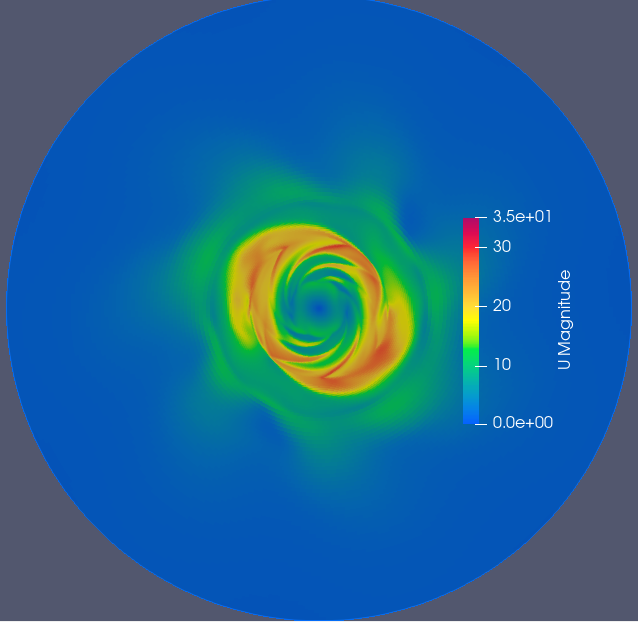
\includegraphics[width=0.5\textwidth]{images/numericalPump/assymetrie.png}
    \caption{Velocity field for Dx = 4e7 and Dy = 2e7}
    \label{fig:assymetry}
\end{figure}



\begin{figure}[H]
    \centering
    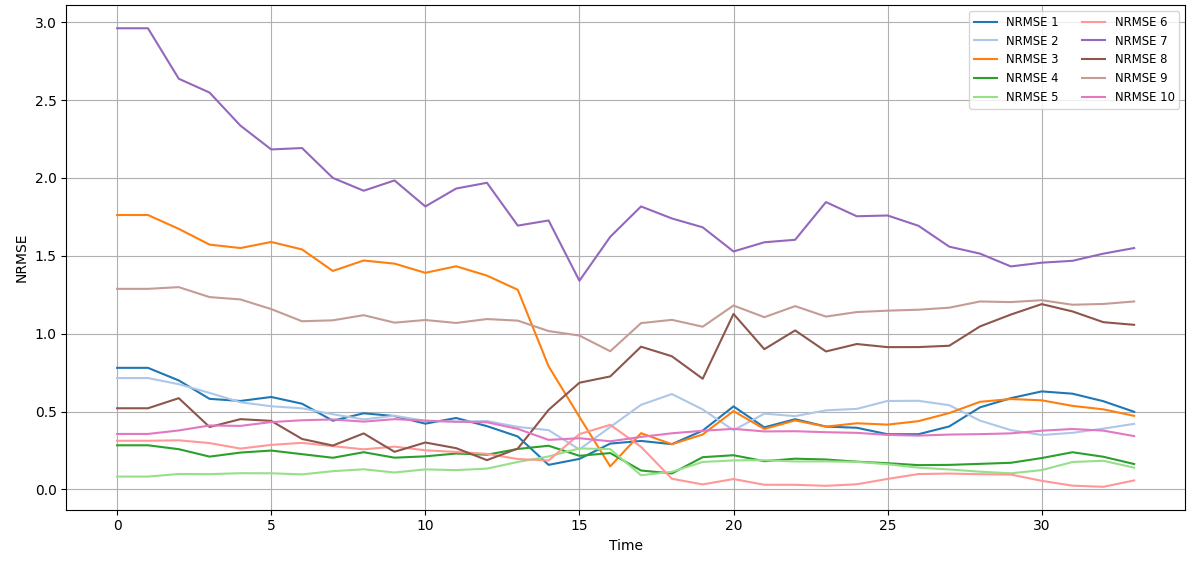
\includegraphics[width=0.5\textwidth]{images/UpdtC14_10NMRSE.png}
    \caption{Evolution of the NRMSEs over EnKF analysis phases}
    \label{fig:UpdtC14_10NMRSE}
\end{figure}


\dots

Explication des écarts par différentes choses 


Tt ce que j'ai implémenté en plus (déjà détaillé partie précédente normalement)

\begin{figure}[H]
    \centering
    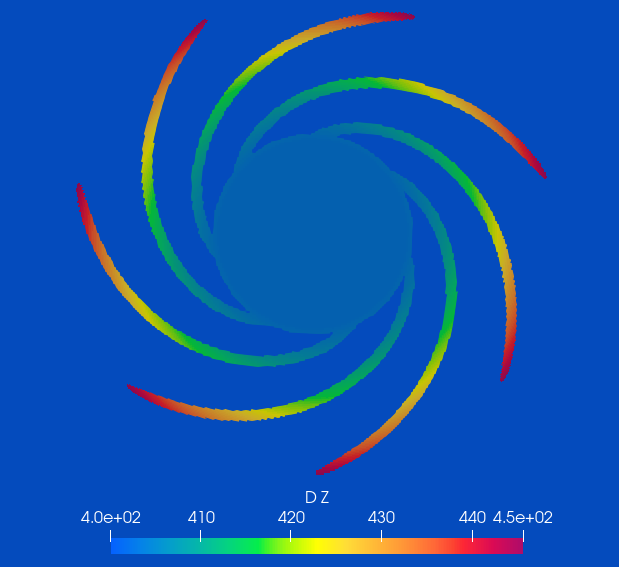
\includegraphics[width=0.5\textwidth]{images/numericalPump/radialExpension.png}
    \caption{Radial expension of Dz over the impeller radius}
    \label{fig:radialExpension}
\end{figure}



Essayer d'améliorer le rendu de l'image ci-dessous en mettant la pompe en transparence
\begin{figure}[H]
    \centering
    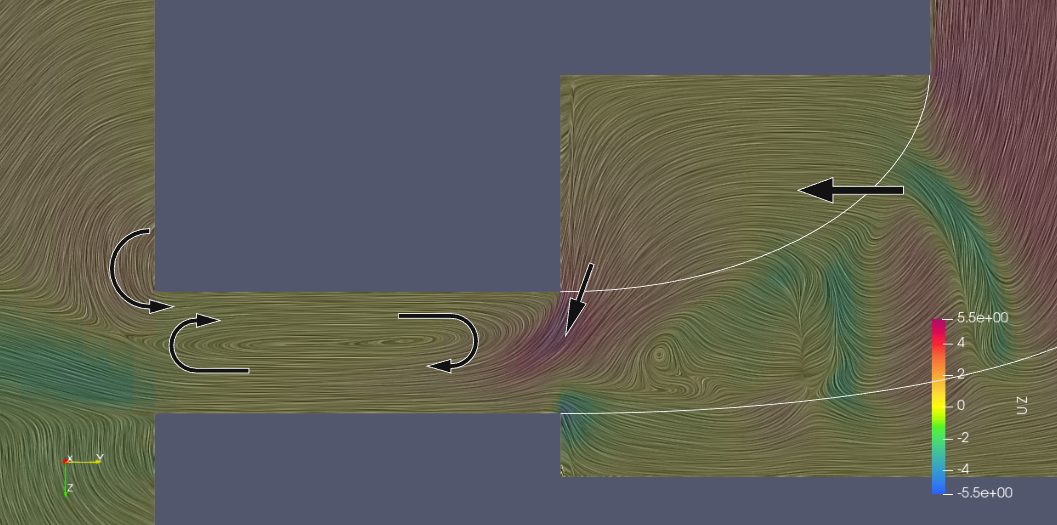
\includegraphics[width=0.5\textwidth]{images/numericalPump/LIC.png}
    \caption{Formation of the recirculation bubble in the diffuser}
    \label{fig:LIC}
\end{figure}

Explication des écarts par la bulle de recirculation.

\subsection{Conclusion ans perspective}

Problème de méthode et pas de miracle ave cette méthode IBM. Interpolation, instationnaire (avantage : on ne contraint plus avec MRF et donc plus facile de réconcilier solution numérique physique et mathématique)


Ouverture : méthode IBM interpolation, article non référencé.

\cite{valeroEnhancedStateEstimation2025} -> ML turbulent channel flow Miguel

"Ouverture / idée" : DA temps réel dans avion impossible pour encore longtemps.
Solution : Contrôle actif de la puissance en fonction des mesures de pression dans le compresseur :
f(obs) -> controle de la puissance
Pour ça, se ref au sujet de thèse de Tarane
obs pression --> modèle de reconstruction du champ de vitesse --> modèle de reconaissance de patternes de décrochage --> contrôle de la puissance
Peut-être faire deux filtres de Kalman imbriqués ? hyperparamètres type fenetre observation, variance initiale, ...



Voir "TD -> Done et "TDSave -> Done" pour voir tt ce que j'ai fais


The random variations are random but with a reproducibility seed (sed) that allows to have the same result each time the simulation is launched.

\newpage

\chapter*{Conclusion}
\addcontentsline{toc}{chapter}{Conclusion}
\vspace{-0.5cm}
%L'objectif de ce stage était d'implémenter une méthode d'\textbf{interpolation linéaire} dans \textbf{Antares} puis de comparer sa précision avec la \textbf{méthode IDW} dans le cas de propagation acoustique avec l'analogie FWH, tout en optimisant la vitesse d'exécution du code.
%Premièrement, une recherche documentaire sur les méthodes d'interpolation implémentables dans notre cas a été menée.
%Ensuite, la méthode linéaire a été implémentée en utilisant une méthode particulière pour les cellules non triangulaires ou rectangulaires.
%L'efficacité a été augmentée dans les cas multi-instants partagés en évitant le recalcule des coefficients d'interpolation à chaque itération. Ces mêmes coefficients peuvent être récupérés par l'utilisateur qui voudrait appeler deux fois le traitement pour une base ayant une même structure.
%La méthode linéaire a été testée sur des cas simples et industriels. Elle fonctionne correctement sur tous les types de cellules, sauf dans certains cas très complexes comme des prismes ayant des faces opposées de tailles différentes et/ou non parallèles.
%Dans le cas de l'aéroacoustique, la méthode linéaire est plus précise que IDW dans tous les cas testés. Cependant, des résultats expérimentaux ont montré que des coefficients (\(N\), \(p\)) autour de (10, 10) donnaient de très bons résultats. Dans ce cas, IDW peut s'avérer plus précis que la méthode linéaire.


%The goal of this internship was to optimise the numerical performance of a centrifugal pump using DA.
%After preparing the experimental data and adapted the OpenFoam solver and CONES code, data was able to be assimilate by the EnKF.
%First results was not convincing, because a recirculation bubble still present in the diffuser. Few more implementation didn't allow the reciculation bubble to break.
%Then, ...


\textbf{Technical and human review}
% ///// Reprendre les objectifs définis à la fin de la section 2.1 //////

%Bilan technique et humain. Liez chaque aspect technique à un aspect humain. Ne traitez pas tout ce qui est technique d’un côté et tout ce qui relève de l’humain d’un autre. Réflexion personnelle sur les spécificités de l’entreprise, du secteur d’activité et du métier que vous avez découverts.

The first thing that I discovered during this internship is the laboratory environment, which is different from a company. The work is more focused on research, and there is a lot of freedom to explore new ideas and methods. The team is very collaborative and supportive, and I learned a lot from my colleagues. I also discovered the importance of communication and documentation in a research environment, as it is essential to share knowledge and results with others. There are still similaritys with a company, such as the social and environmental responsibility, that I presented in a first part.

After having done a state of art on the topics, we saw that the DA method is a good candidate to DNS or costly LES, for industrial applications, because it allows to have a good accuracy with a lower computational cost. I saw that an international expertise on application relies on this topic has been developed in the last few years on the laboratory. Numerical ingredients and usefull libraries were presented. The state of art was a good opportunity to learn more about the DA method and its applications. It was not too hard because most of information were already known by the laboratory. I also learned a lot about the IBM method and its applications, which is a good alternative to the traditional methods for the simulation of complex geometries.

Then, an explanation of the pump modeling, the pre-processing of the experimental data and the implementation of the IBM method in OpenFOAM were given. The redaction of this part helps me to structure my thoughts and to better understand the different steps of the pre-processing. I also learned a lot about the IBM method and its implementation in OpenFOAM, which was not easy at the beginning because I had to learn a lot about OpenFOAM and C++ programming. The implementation of the IBM method was a good opportunity to learn more about OpenFOAM and its functionalities.

Finally, we presented the first results of the numerical simulation and the first application of the DA method on the centrifugal pump case.
The results show that the IBM method as applied here does not give us a result consistent with physical observations and the DA does not allow us to improve this result. The solution is not converging and the velocity field is not physical, with a recirculation bubble in the diffuser. Several strategies were tested to try to improve the solution, but none of them allowed to obtain a satisfactory result.

I really enjoyed this internship beacause I learned a lot about all the topics that I love. That is why I decided to continue to work on this topic for my PhD thesis "Combining experimental and numerical techniques for the analysis of axial compressor internal flows using Data Assimilation" in the same laboratory.

%\subsection*{Technical and human review}

\textbf{Outlook}

To continue this work, it would be interesting to try to change the IBM method (try the "interpolation method" for example) or to try an instationnary (URANS or LES) simulation to see if it can overcome these non-physical results.

The DA method is still not widely used in the industry, but it has a lot of potential for the future. The main challenge is to adapt the DA method to the specific needs of the industry, such as the use of complex geometries and the need for real-time applications. I discovered that DA can be long to implement and sometimes difficult to converge. At same time, EnKF needs a huge number of CPUs. Sometimes, I need to wait several days to launch a simulation. It would be interesting to try to reduce the computational cost of the DA method, by using more efficient algorithms or by using machine learning techniques, as presented in the state of art.
The IBM method is a good alternative to the traditional methods for the simulation of complex geometries, because it allows to have a good accuracy with a lower computational cost. An other challenge is to improve the accuracy of the IBM method.

\begin{comment}
J’ai été enthousiasmé par ce stage au CERFACS, à plusieurs titres. Il m’a non seulement permis de développer et renforcer de nombreuses connaissances dans le domaine informatique mais également sur le plan humain. Il m’a donné une belle occasion de découvrir la vie d’un laboratoire de recherche.

L'objectif de ce stage était d'implémenter une méthode d'interpolation linéaire dans Antares puis de comparer sa précision avec la méthode IDW dans le cas de propagation acoustique avec l'analogie FWH, tout en optimisant la vitesse d'exécution du code.
Après avoir exploré la structure d'Antares, une recherche documentaire a été menée pour savoir quelle méthode, implémentable dans la librairie, pouvait être candidate pour compléter la méthode IDW et linéaire. Quelques méthodes polynomiales et géostatistiques ont pu être mises en évidence. Une présentation un plus détaillée de la méthode par voisin le plus proche, IDW et linéaire a aussi été réalisée.
L'un des principaux résultats de ce stage a été l'implémentation globalement réussie de la méthode d'interpolation linéaire, qui s'est révélée  généralement plus précise que la méthode de Pondération Inverse à la Distance (IDW) précédemment codée.
Coder l’interpolation linéaire jusqu’en 3D n’a été ni très difficile, ni chronophage. Cependant, l’intégrer au code déjà existant et faire les tests fut plus délicat. Le soutien de mon maître de stage a été primordial pour me montrer comment fonctionnent les outils au CERFACS et m'aider à sortir d'impasses.
Cette nouvelle méthode a été testée sur des cas académiques mais aussi sur des cas industriels tels que sur une vue en coupe à la position (0, 0, 0.01), selon l'axe z de la chambre de combustion preccinsta.
L'étude sur les coefficients \(N\) et \(p\) de la méthode IDW a montré que pour des paramètres (\(N\), \(p\)) autour de (10, 10) nous pouvons obtenir de meilleurs résultats qu'avec la méthode linéaire, dans le cas d'aéroacoustique étudié.
Ce travail a aussi amélioré les performances du code (cinq fois plus rapide pour la méthode IDW dans un cas test d'aéroacoustique).
Le code ajouté pourrait aussi faciliter l'intégration de méthodes d'ordre supérieur grâce à certaines fonctions python réutilisables.
J'ai ressenti tout au long de mon stage l'importance de réaliser un travail ouvrant des perspectives nouvelles pour un chercheur.
Enfin, ce stage n'a pas été qu'une expérience professionnelle enrichissante. Il a conforté mon intérêt pour les méthodes numériques appliquées et la recherche en calcul scientifique. Je suis particulièrement reconnaissant pour l'accompagnement dont j'ai bénéficié tout au long de cette expérience et pour les opportunités de développement personnel et professionnel qu'il m'a offert.
\end{comment}

%\subsection*{Outlook}
%Pour continuer à améliorer le traitement d'interpolation d'Antares, on pourrait implémenter l'une des méthodes d'ordre supérieur citées dans la section \ref{s223}.
%On pourrait également compléter les tests de la méthode linéaire sur la chaîne aéroacoustique, en observant la polaire de l'amplitude en fonction de l'observateur dans le cas d'un Mac non nul.
%Afin d'améliorer la rapidité, le code pourrait être passé en parallèle pour pouvoir s’exécuter sur plusieurs processeurs à la fois.
%Une petite amélioration qui permettrait de rendre le code compatible avec plus de bases serait d'inclure les bases "multizones" à l'interpolation linéaire.
% Faire la ref


%\subsection*{Personal reflection}


%Le CERFACS est un laboratoire privé à la pointe des simulations numériques. Il s'est d'abord spécialisé dans l'aérodynamique et s’intéresse maintenant de plus en plus à la combustion. Il adapte ses domaines de recherche aux domaines importants de l'industrie.
%Durant ce stage, au-delà des aspects techniques, j'ai eu un bel aperçu du métier de chercheur tant au travers de mes missions que dans mes rencontres. Il s'agit de rechercher et de s'appuyer sur le travail déjà réalisé autour de notre problématique.
%Ensuite, il faut explorer des pistes qui peuvent s'avérer infructueuses après les avoir longuement explorées.
%Enfin, un travail de rédaction est nécessaire pour expliquer clairement notre travail aux scientifiques.
\newpage

\newpage
\listoffigures

\newpage
\chapter*{Table des annexes}
\addcontentsline{toc}{chapter}{Table des annexes}

\begin{itemize}
    \item \textbf{Annexe 1} – Batch code used to run simulation on the Rome partition of TGCC cluster \dotfill \pageref{annex:BatchCode}
    \item \textbf{Annexe 2} – OpenFOAM Directory Tree \dotfill \pageref{annex:OpenFoamArbo}
    % Ajoute ici les autres annexes au fur et à mesure
\end{itemize}
\newpage


\newpage
\input{annexes/annexes.tex}
\newpage

\nocite{*}
\printbibliography
\addcontentsline{toc}{chapter}{Bibliography}
\newpage

\printacronyms[name=List of acronyms, heading=chapter*]
\addcontentsline{toc}{chapter}{List of acronyms}
\label{sec:glossary}

\cleardoublepage

\large{\textbf{Résumé / Abstract}}

\vspace{0,5cm}

\paragraph{Résumé}

Ce stage de fin d'études cloture mon cursus à l'IPSA Toulouse.
Il a été réalisé au Laboratoire de Mécanique des Fluides de Lille (LMFL), sur le campus de l'Ecole National des Arts et Métiers. En s'appuyant sur les traveaux déjà présents dans la littérature, notament au LMFL, l'objectif du stage intitulé \textit{Optimisation des performances d'une pompe centrifuge à l'aide de l'assimilation de données} était de faire de l'\textbf{Assimilation de Données} en utilisant la librairie d'\textbf{CONES} pour combiner des simulations \textbf{OpenFOAM} avec des données prise sur une \textbf{pompe centrifuge} au LMFL. Cela dans l'objectif d'améliorer la simulation numérique utilisant une méthode aux frontière immergés (IBM). La méthode choisie pour l'assimilation des données est le \textbf{filtre de Kalman d'ensemble (EnKF)}, qui permet de combiner les données de simulation et les observations expérimentales pour obtenir une estimation plus précise de l'état du système. Les résultats obtenus montrent un défault de la méthode IBM dans la zone du diffuseur, qui n'a pas pu être corrigé par l'assimilation de données. Cependant, l'implémentation de l'EnKF dans CONES a bien été réalisé et des perspectives d'amélioration ont été identifiées pour corriger ce défault.
Ce stage ouvre sur une thèse que je commencerais en octobre 2025 au LMFL, sur un sujet similaire.

\begin{comment}
L'objectif de ce stage était d'implémenter une méthode d'\textbf{interpolation linéaire} dans \textbf{Antares} puis de comparer sa précision avec la \textbf{méthode IDW} dans le cas de propagation acoustique avec l'analogie FWH, tout en optimisant la vitesse d'exécution du code.
Premièrement, une recherche documentaire sur les méthodes d'interpolation implémentables dans notre cas a été menée.
Ensuite, la méthode linéaire a été implémentée en utilisant une méthode particulière pour les cellules non triangulaires ou rectangulaires.
L'efficacité a été augmentée dans les cas multi-instants partagés en évitant le recalcule des coefficients d'interpolation à chaque itération. Ces mêmes coefficients peuvent être récupérés par l'utilisateur qui voudrait appeler deux fois le traitement pour une base ayant une même structure.
Le code est jusqu'à \(n\) fois plus rapide pour une base ayant \(n\) instants partagés.
La méthode linéaire a été testée sur des cas simples et industriels. Elle fonctionne correctement sur tous les types de cellules, sauf dans certains cas très complexes comme des prismes ayant des faces opposées de tailles différentes et/ou non parallèles.
Dans le cas de l'aéroacoustique, la méthode linéaire est plus précise que IDW dans tous les cas testés. Cependant, des résultats expérimentaux ont montré que des coefficients (\(N\), \(p\)) autour de (10, 10) donnaient de très bons résultats. Dans ce cas, IDW peut s'avérer plus précis que la méthode linéaire.
\end{comment}

Mots-clés: \textbf{Assimilation de Données, OpenFOAM, CONES, Pompe centrifuge, filtre de Kalman d'ensemble (EnKF), méthode aux frontière immergés (IBM)}

\paragraph{Abstract}
\vspace{0,5cm}

This end-of-studies internship concludes my curriculum at IPSA Toulouse.
It was carried out at the Fluid Mechanics Laboratory of Lille (LMFL), on the campus of the Ecole National des Arts et Métiers. Building on previous work in the literature, notably at LMFL, the objective of the internship entitled \textit{Optimization of the performance of a centrifugal pump using Data Assimilation} was to perform \textbf{Data Assimilation} using the \textbf{CONES} library to combine \textbf{OpenFOAM} simulations with data taken on a \textbf{centrifugal pump} at LMFL. The goal was to improve the numerical simulation using an \textbf{Immersed Boundary Bethod (IBM)}. The chosen method for data assimilation is the \textbf{Ensemble Kalman Filter (EnKF)}, which allows to combine simulation data and experimental observations to obtain a more accurate estimate of the state of the system. The results obtained show a flaw in the IBM method in the diffuser area, which could not be corrected by data assimilation. However, the implementation of the EnKF in CONES was successfully carried out and improvement perspectives were identified to correct this flaw.
This internship opens the way to a PhD that I will start in October 2025 at LMFL, on a similar subject.     

Keywords: \textbf{Data Assimilation, OpenFOAM, CONES, Centrifugal pump, EnKF, IBM}


\begin{comment}

The objective of this internship was to implement a \textbf{linear interpolation} method in \textbf{Antares} and then to compare its accuracy with the \textbf{IDW method} in the case of acoustic propagation using the FWH analogy, while optimizing the code execution speed.
First, a literature review on interpolation methods applicable to our case was conducted.
Secondly, the linear method was implemented using a special method for non-triangular or rectangular cells.
Efficiency was increased in shared multi-instant cases by avoiding the recalculation of interpolation coefficients at each iteration.
These same coefficients can be reused by a user who wants to run the process twice on a base with the same structure.
The code is almost \(n\) times faster for a database with \(n\) shared instants.
The linear method has been tested on simple and industrial cases.
It works correctly on all cell types, except in some very complex cases, such as prisms with non-parallel and/or differently sized opposing faces.
In the case of aeroacoustics, the linear method is more accurate than IDW in all tested scenarios. However, experimental results have shown that coefficients (\(N\), \(p\)) around (10, 10) produce very good results. In such cases, IDW may prove to be more accurate than the linear method.
\end{comment}

\begin{comment}
    Ce rapport de stage présente le travail effectué au \textbf{CERFACS}, un institut de recherche axé sur le calcul haute performance (HPC).

    Destiné à l'\textbf{IPSA}, ainsi qu'aux utilisateurs et développeurs du code d'\textbf{interpolation} de la \textbf{librairie Antares} utilisée pour le post-traitement de simulations numériques, ce document propose une vue d'ensemble des activités menées.

    Il débute par une présentation générale du CERFACS, avant de détailler le stage.
    Ce dernier inclut une introduction à la librairie Antares et à son utilisation pour l'interpolation, suivie d'un état de l'art des différentes méthodes d'interpolation susceptibles d'être intégrées dans la librairie.
    Une description de l'implémentation de la méthode linéaire est ensuite fournie, avec un focus sur les optimisations réalisées.
    Enfin, les résultats de la comparaison entre la méthode de \textbf{Pondération Inverse à la Distance} (IDW) précédemment codée et la \textbf{méthode linéaire} implémentée sont exposés.

    \paragraph{Abstract}

    \vspace{0,5cm}

    This internship report presents the work carried out at \textbf{CERFACS}, a research institute focused on High-Performance Computing (HPC).

    Intended for the \textbf{IPSA}, as well as the users and developers of the \textbf{interpolation} code in the \textbf{Antares library} used for post-processing numerical simulations, this document provides an overview of the activities undertaken.

    It begins with a general presentation of CERFACS, followed by a detailed account of the internship.
    The latter includes an introduction to the Antares library and its use for interpolation, followed by a state-of-the-art review of various interpolation methods that could potentially be integrated into the library.
    A description of the implementation of the linear method is then provided, with a focus on the optimizations performed.
    Finally, the results of the comparison between the previously coded \textbf{Inverse Distance Weighting} (IDW) method and the implemented \textbf{linear method} are presented.
\end{comment}



\end{document}
